\chapter{Transcutaneous \texorpdfstring{\gls{co2}}{CO2} Sensing}\label{chap:tcco2}

\begin{tldrbox}
	
	Given the failure of the spectrophotometric approach envisioned in the previous chapter, the remainder of this doctoral work focuses solely on transcutaneous \gls{co2} sensing. To perfect this latter approach, it was necessary to better understand the specificities of transcutaneous \gls{co2} measurement. More specifically, this chapter delves into the following processes:
	\begin{enumerate}
		\item Constructing a mathematical model to determine the factors that influence the response time of such a sensor. This response time is ultimately dependent on two elements: the skin's conductivity towards \gls{co2} and the sensor's equivalent height---\ie{} its internal volume divided by its contact surface with the skin.
		\item Characterising the latter conductivity, and its dependence on skin temperature in particular. A clinical study was conducted on 40 subjects, showing that \emph{not} heating the skin would be acceptable from a response time point of view. This study also provided evidence that doing so might lead to \gls{ptco2} values that are close enough to \gls{paco2} from a clinical point-of-view.
		\item Pinpointing the environmental conditions of cutaneous sensing, which can me summarised as follows: a temperature in the 32--34{\degree}C range without external clothing---35{\degree}C with---and humidity levels in the 80--100\% \gls{rh} range. The skin itself is also highly hypoxic---but \gls{o2} is still present---and acidic.
	\end{enumerate}
	
	Taken together, these insights provides a useful framework for the development of future \gls{ptco2} sensors, as described in the following chapters.
	
	\tcblower
	
	\hyperref[chap:co2hb]{Previous chapter} \hfill \hyperref[chapter:toc]{Main Table Of Content (TOC)} \hfill \hyperref[chap:choosing_techno]{Next chapter}
	
\end{tldrbox}

As mentioned in \hyperref[chap:intro]{the introduction}, the many limitations of current \gls{ptco2} monitors combined with the unfeasibility of pulse carbametry both call for a new generation of transcutaneous \gls{co2} sensors to be developed. To this end, it is necessary to better understand the specificities of transcutaneous \gls{co2} sensing, in particular by addressing the following questions:
\begin{enumerate}
	\item How can the working principles of equilibrium-based \gls{ptco2} sensors be modelled? And what key figures of merit are important to consider when designing such a sensor?
	\item What are the specificities of transcutaneous \gls{co2} diffusion? In particular, what is the influence of skin temperature on the skin conductivity towards \gls{co2}?
	\item What factors influence the final \gls{ptco2} value at equilibrium? In particular, what is the influence of skin temperature on the \gls{paco2} / \gls{ptco2} correlation?
	\item What conditions---temperature, humidity, acidity or ionic content---can be expected at the skin?
\end{enumerate}

This first aspect is addressed in Section~\ref{sect:tcco2:modelling_tc_sensing}, which is strongly inspired by the Section~4.2 and Supplementary Materials of our\footnote{There again, and in the corresponding sections, the first person plural was chosen since those are collective works, whose authorship I share with my co-authors.} 2022 Sensors review article\cite{dervieux2022}. The second and third aspects are then discussed in Section~\ref{sect:tcco2:frontiers_article}, based on our 2023 Frontiers in Physiology paper\cite{dervieux2023rate}. Finally, the fourth aspect is treated in Section~\ref{sect:tcco2:skin_conditions}.

\section{Modelling Equilibrium-Based \texorpdfstring{\gls{ptco2}}{tcpCO2} Sensing}\label{sect:tcco2:modelling_tc_sensing}

This first section focuses on studying the transcutaneous diffusion of \gls{co2} using a simple skin and equilibrium-based sensor model. After presenting the said model in Section~\ref{sect:tcco2:model} and briefly discussing the influence of the sensor's chamber nature in Section~\ref{sect:tcco2:inner_medium}, the dynamic of \gls{ptco2} measurements is derived in Section~\ref{sect:tcco2:diffusion_dynamic}. Finally, the existing literature is reviewed to estimate the achievable response times for future \gls{ptco2} sensors in Section~\ref{sect:tcco2:response_time}. Of note, the perceptive reader may wonder why the emphasis is placed on \emph{equilibrium-based} sensing in the present work. This is to distinguish it from another modality of \gls{ptco2} sensing, called \emph{rate-based} sensing, which has been investigated by some authors. Although largely beyond the scope of my research, this alternative sensing technique is briefly mentioned in Section~\ref{subsect:choos:pot:rate_based}.

\subsection{The Model}\label{sect:tcco2:model}

The model of transcutaneous \gls{co2} sensing that is considered in all subsequent developments is presented in Figure~\ref{fig:tcco2:diffusion_model}. In this model, the subcutaneous tissues are considered as a homogeneous, semi-infinite medium occupying the $x\leq 0$ space volume. The subcutaneous tissues can be thought of as a \gls{co2} reservoir with a constant partial \gls{co2} pressure equal to \gls{ptco2}. Between $x=0$ and $x=w$ is the skin membrane, of thickness $w$ and diffusivity $D$ (m$^2$.s$^{-1}$) towards \gls{co2}. In this skin model, the sub-cutaneous tissues and skin barrier are only used as a representation, and the skin barrier does \textbf{not} represent literally the stratum corneum. Consequently, the $w$ and $D$ parameters can hardly be measured experimentally since they are mere model parameters---see Section~\ref{sect:tcco2:k_metric_choice} for a more detailed discussion on this topic.

\begin{figure}
	\centering
	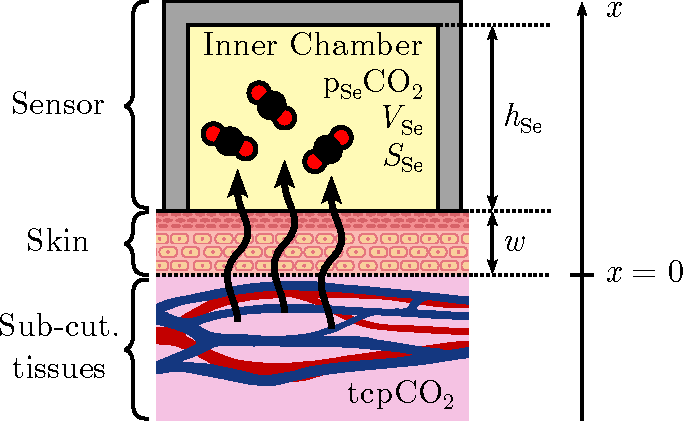
\includegraphics[scale=0.7]{1_main_matter/tcco2_figures/diffusion_model.pdf}
	\caption{Simplified model of \gls{co2} diffusion through the skin inside a closed sensor.}
	\label{fig:tcco2:diffusion_model}
\end{figure}

On top of these two layers is positioned a sensor consisting in an inner sensing medium of volume $V_\text{Se}$, surface in contact with the skin $S_\text{Se}$ and height $h_\text{Se} = V_\text{Se} / S_\text{Se}$. This sensor is in turn surrounded by a gas-tight enclosure that prevents gaseous exchanges between the sensing medium and the outside---except for those with the skin surface, of course.

\subsection{Inner Sensing Medium}\label{sect:tcco2:inner_medium}

In the calculations conducted throughout the next sections, the inner sensing medium is always considered as an homogenous air volume. While this assumption is more than justified in the case of \gls{ndir} or (photo-)acoustic sensors, it seems more debatable in the case of conductometric or dye-based sensors---these different types of sensors are reviewed in Chapter~\ref{chap:choosing_techno}. Yet, every sensing medium can be viewed as a potential \gls{co2} reservoir through Henry's law, and thus be considered as an equivalent air volume.

For instance, if the sensing medium is water---\eg{} in the case of a wet conductometric sensor---with a water volume $V_\text{water}$ of height $h_\text{water}$, this latter water volume is equivalent to an air volume $V_\text{air,eq}$ of height $h_\text{air,eq}$ such that the amount of \gls{co2} dissolved in the water volume $n_\text{\gls{co2},water}$ (mol) is the same as that in an equivalent air volume $n_\text{\gls{co2},air,eq}$ for a given \gls{pco2}, \ie{}
\begin{equation}
	n_\text{\gls{co2},air,eq}(\text{\gls{pco2}}) = n_\text{\gls{co2},water}(\text{\gls{pco2}})
\end{equation}
with
\begin{equation}
	\begin{aligned}
		&n_\text{\gls{co2},air,eq}(\text{\gls{pco2}}) = \frac{\text{\gls{pco2}} \cdot V_\text{air,eq}}{R\cdot T} \quad \text{(ideal gas law)}\\
		&\ce{[CO_{2,water}]} = K_s \cdot \text{\gls{pco2}} \quad \text{(Henry's law)}\\
		&n_\text{\gls{co2},water}(\text{\gls{pco2}}) \triangleq V_\text{water} \cdot \ce{[CO_{2,water}]}\\
		&V_\text{water} = S_{Se} \cdot h_\text{water} \quad \text{and} \quad V_\text{air,eq} = S_{Se} \cdot h_\text{air,eq}\\
	\end{aligned}
\end{equation}
wherein $R$ is the ideal gas constant (J.K$^{-1}$.mol$^{-1}$), $T$ the temperature (K) and $K_s$ (mol.m$^{-3}$.Pa$^{-1}$) is the solubility of \gls{co2} in water---see \eg{} Weiss\cite{weiss1974} for numerical values of $K_s$. Combining the above equations yields
\begin{equation}
	h_\text{air,eq} = h_\text{water} \cdot R \cdot T \cdot K_s
\end{equation}

Taking Weiss' value for $K_s$ in pure water at 293~K under 1~atm yields
\begin{equation}
	h_\text{air,eq} \approx 0.952 \cdot h_\text{water}
\end{equation}
% k0 = 3.910e-2 mol/L/atm, r*t*k0*1e3/1e5 (L->m3, atm->Pa)
and a similar train of thought can be applied to other media. Thanks to Henry's law, it is thus theoretically always possible to convert from a given sensing medium into an equivalent air volume as is done above for water.

Of note, one should bear in mind that the afore considerations are especially true if the \gls{co2} diffusion process into the sensing medium is also neglected. Indeed, it is assumed in the remainder of this chapter that as soon as \gls{co2} crosses the skin barrier and reaches the sensing medium itself, it readily diffuses into it. Thus the \gls{pco2} inside the sensing medium is considered to be homogenous and only dependent on the amount of \gls{co2} having diffused through the skin. This assumption is more than justified in first approximation when considering the response times of the different sensing techniques presented in Chapter~\ref{chap:choosing_techno}. Indeed, most of them easily reach response times below 1~min, which is far below the response times of the simple model presented in Section~\ref{sect:tcco2:response_time} for thicknesses $h_{Se}$ in the order of 100~\textmu{}m, or above.

\subsection{Diffusion Through the Skin}\label{sect:tcco2:diffusion_dynamic}

The \gls{co2} diffusion across the skin barrier can be studied using Fick's first law of diffusion:
\begin{equation}
	J_S = -D \cdot \frac{d \ce{[CO_2]}(x)}{dx}
\end{equation}
wherein $J_S$ is the \gls{co2} diffusion flux per unit area (mol.m$^{-2}$.s$^{-1}$), $D$ the diffusivity of skin toward \gls{co2} (m$^2$.s$^{-1}$), and \ce{[CO_2]} the \gls{co2} concentration (mol.m$^{-3}$) inside the skin membrane itself. With the hypothesis ($\mathcal{H}_1$) that there is no \gls{co2} accumulation inside the skin itself---\ie{} that the capacitive effect of the skin is negligible compared to that of the sensing medium---$J_S$ can be considered constant along the $x$ axis, leading to:
\begin{equation}\label{eq:tcco2:fick_int}
	J_S = \frac{D}{w} \cdot \left( \ce{[CO_2]}(x=0) - \ce{[CO_2]}(x=w)  \right)
\end{equation}

Since $x=0$ corresponds to the subcutaneous tissues---wherein \gls{pco2} = \gls{ptco2}---and $x=w$ corresponds to the inner sensing medium---wherein \gls{pco2} = \gls{pseco2}---we have
\begin{equation}\label{eq:tcco2:conc_boundaries}
	\begin{cases}
		\ce{[CO_2]}(x=0) = K_\text{skin,\ce{CO_2}} \cdot \text{\gls{ptco2}}\\
		\ce{[CO_2]}(x=w) = K_\text{skin,\ce{CO_2}} \cdot \text{\gls{pseco2}}
	\end{cases}
\end{equation}
wherein $K_\text{skin,\ce{CO_2}}$ is the solubility of \gls{co2} into the skin (mol.m$^{-3}$.Pa$^{-1}$). Besides, under ($\mathcal{H}_1$):
\begin{equation}\label{eq:tcco2:fluxes_int}
	\frac{d n_\text{\ce{CO_2}, Se}}{dt} = S_\text{Se} \cdot J_S 
\end{equation}
wherein $n_\text{\ce{CO_2}, Se}$ is the amount of \gls{co2} in the inner sensing medium (mol), given by:
\begin{equation}\label{eq:tcco2:id_gas}
	n_\text{\ce{CO_2}, Se} = \frac{\text{\gls{pseco2}} \cdot V_\text{Se}}{R \cdot T} \quad \text{(ideal gas law)}
\end{equation}

Equations \ref{eq:tcco2:fick_int}--\ref{eq:tcco2:id_gas} then yield:
\begin{equation}
	\frac{d \text{\gls{pseco2}}}{dt} = \frac{D}{w \cdot h_\text{Se}} \cdot R \cdot T \cdot K_\text{skin,\ce{CO_2}} \cdot \left( \text{\gls{ptco2}} - \text{\gls{pseco2}} \right)
\end{equation}

Additionally, $K_\text{skin,\ce{CO_2}}$ can be estimated from the solubility of \gls{co2} in various biological tissues\cite{wright1934, nichols1957, scheuplein1976, gill1988} leading to an $R\cdot T\cdot K_\text{skin,\ce{CO_2}}$ factor in the 0.6--1.0 range. Close to these values, Scheuplein \etal{}\cite{scheuplein1976} present an $R\cdot T\cdot K_\text{skin,\ce{CO_2}}$ product near 1.5 for the stratum corneum. Again though, the skin membrane of the afore-presented model does not necessarily represent the stratum corneum alone, but is only a model for the different skin layers that may hinder \gls{co2} diffusion. Consequently, I chose to take the dimensionless $R\cdot T\cdot K_\text{skin,\ce{CO_2}}$ product equal to 1 in the following developments. Another possibility would be to simply integrate its value inside the $w/D$ ratio, leading to identical conclusions in the end, at the cost of an additional complexity in the notations. Discarding it yields the following simplified differential equation
\begin{equation}
	\frac{d \text{\gls{pseco2}}}{dt} = \frac{D}{w \cdot h_\text{Se}} \cdot \left( \text{\gls{ptco2}} - \text{\gls{pseco2}} \right)
\end{equation}
which---considering the initial condition \gls{pseco2}$(t=0)=0$---has a unique solution:
\begin{equation}\label{eq:tcco2:pseco2_full_mod}
	\text{\gls{pseco2}}(t) = \text{\gls{ptco2}} \cdot \left( 1 - e^{-\frac{t}{\tau}} \right), \quad \text{with } \tau = h_{Se} \cdot \frac{w}{D}
\end{equation}

This formulation is essentially the same as that derived by Chatterjee \etal{}\cite{chatterjee2015}, although they used a more sophisticated model taking into account the \gls{co2} production inside the skin, leading to an additional $\beta/\alpha$ factor in Equation~6 of their work. Equation~\ref{eq:tcco2:pseco2_full_mod} describes a classical first-order response, as can be seen in Figure~\ref{fig:tcco2:response_time}, Left, with a 95\% response time Tr$_{95\%}\approx 3\cdot \tau = 3 \cdot h_\text{Se} \cdot w / D$. It is important to note at this point that only the equivalent height $h_\text{Se}$ of the sensor really matters from a response time point of view. The actual inner volume of the sensor may indeed be convoluted---\ie{} have a non-prismatic shape---only its volume to surface ratio $h_\text{Se}$ comes into play in the above considerations.

\begin{figure}
	\centering
	\includegraphics[width=.95\linewidth]{1_main_matter/tcco2_figures/tikz/out/response_time.pdf}
	\caption[Influence of a transcutaneous sensor's height on its response time.]{95\% response time ($Tr_{95\%} \approx 3\cdot \tau$) for a sensor of height $h_{Se}$. The blue area underlines the portion of the line with a response time below 10~min, which corresponds to a sensor height below approximately 100~\textmu{}m.}
	\label{fig:tcco2:response_time}
\end{figure}

\subsection{Response Time}\label{sect:tcco2:response_time}

As mentioned in Section \ref{sect:tcco2:model}, the $w$ and $D$ parameters cannot be measured experimentally since they are only model parameters. However, the $w/D$ fraction can be estimated from the \gls{co2} exhalation rate through the skin per unit area---$Q$ (m$^{3}$.m$^{-2}$.s$^{-1}$)---defined as
\begin{equation}
	Q = \frac{1}{S_\text{Se}} \cdot \frac{d V_\text{\gls{co2},Se}}{dt}
\end{equation}
wherein $V_\text{\gls{co2},Se}$ is the volume that would occupy the amount of \gls{co2} contained inside the sensing medium if it were subjected to a total ambient pressure p$_0$. It is given by
\begin{equation}
	\frac{V_\text{\gls{co2},Se} }{V_\text{Se}} = \frac{\text{\gls{pseco2}}}{\text{p}_0}
\end{equation}

yielding:
\begin{equation}
	Q = \frac{h_\text{Se}}{\text{p}_0} \cdot \frac{d \text{\gls{pseco2}}}{dt}
\end{equation}

Taking the first derivative of \gls{pseco2}---see Equation \ref{eq:tcco2:pseco2_full_mod}---with respect to time, and evaluating it at $t=0$ leads to
\begin{equation}
	\tau = \frac{h_\text{Se}}{Q} \cdot \frac{\text{\gls{ptco2}}}{\text{p}_0} \quad \text{or} \quad \frac{w}{D} = \frac{\text{\gls{ptco2}}}{Q \cdot \text{p}_0}
\end{equation}

Several works on the determination of $Q$ for \gls{co2} across human skin can be found in the literature---see Table~\ref{table:tcco2:diff_rate_lit}, below---and a value of 100~cm$^3$.m$^{-2}$.h$^{-1}$ can reasonably be assumed. Since the afore-mentioned works concern healthy subjects, we can also assume a normal capnia of 5.3~kPa (or 40~mmHg)\cite{geers2000}. In these conditions, and with p$_0 = 1$~atm:

\begin{equation}
	\frac{w}{D} \approx 1.90\times10^6~\text{s.m$^{-1}$}
\end{equation}

To illustrate this value, if the sensor's height were 1~mm, $\tau$ would be near 1900~s, or about 32~min, and a 95\% response would be reached after 1~h~35~min---or $3\cdot \tau$. By contrast, a more realistic response time---and, more importantly, one that would be clinically usable---of below 10 minutes would require a thickness of less than 100~{\textmu}m, as can be seen in Figure~\ref{fig:tcco2:response_time}, Right.

\textbf{Note:} $Q$ is of course time-dependent, especially during transcutaneous monitoring with the presented closed-chamber sensor model---as it will decrease with a diminishing \gls{ptco2} / \gls{pseco2} gradient. However, since only its value at $t=0$ has been used in the end in the above development, and since it is also the only $Q$ value reported in the literature, the $Q(t)$ notation was neglected.

\subsection{Consequences for the Design of Future \texorpdfstring{\gls{ptco2}}{tcpCO2} Sensors}

The response time of the sensor introduced in the above model is thus only a function of two elements:
\begin{enumerate}
	\item the dimensions of the sensor itself, and more specifically the equivalent height $h_{Se}$ of its sensing chamber, \ie{} the $V_\text{Se}/S_\text{Se}$ ratio---as mentioned in Section~\ref{sect:tcco2:diffusion_dynamic}---and
	\item the properties of the skin membrane, and more specifically its thickness and diffusivity towards \gls{co2}---\ie{} the $w/D$ ratio.
\end{enumerate}

Quite intuitively, a large surface to volume ratio for the sensing chamber, a thin skin membrane and an elevated skin diffusivity towards \gls{co2} all lead to a faster sensor. Consequently, in order to decrease the response time of a transcutaneous \gls{co2} sensor, one can either act on the sensor's form factor---by designing a thinner sensor---or on the skin diffusivity and thickness. While choosing a \gls{co2} sensing technique with a compact form factor is at the very heart of Chapter~\ref{chap:choosing_techno}, the next section focuses on the skin diffusivity towards \gls{co2}. More specifically, several authors reported an increasing transcutaneous \gls{co2} exhalation rate with an increasing temperature\cite{shaw1929, shaw1930, whitehouse1932}. However, the latter temperature was often that of the ambient air surrounding the skin, and not that of the skin itself. I thus decided to lead a thorough clinical study on this very topic, which is the object of the next section. As a side note, this study also led me to take an interest in skin stripping---\ie{} thinning the skin---and its impact on the transcutaneous \gls{co2} exhalation rate---see Section~\ref{sect:tcco2:q_metric_choice}.

\section[Skin Temp. Influence on Tc. \texorpdfstring{\gls{co2}}{CO2} Conductivity]{Skin Temperature Influence on Transcutaneous \texorpdfstring{\gls{co2}}{CO2} Conductivity and Skin Blood Flow}\label{sect:tcco2:frontiers_article}

Of note, this section is essentially a slightly revised\footnote{In particular, a large part of the introduction of the original article has been omitted.} version of the article entitled \textit{Skin temperature influence on transcutaneous carbon dioxide (CO$_\textit{2}$) conductivity and skin blood flow in healthy human subjects at the arm and wrist}, and published in the Frontiers in Physiology journal in late 2023\cite{dervieux2023rate}.

\subsection{Introduction}\label{sect:tcco2:frontiers_intro}

It stems from the above that developing a new generation of \gls{ptco2} sensors requires to address the two following issues:
\begin{enumerate}
	\item First, in order to dimension the sensor-to-be, it is essential to accurately know the \gls{co2} \emph{exhalation rate} through the skin, as the latter directly influences the response time of the sensor.
	\item Then, it is mandatory that the \gls{ptco2} and \gls{paco2} be in good agreement at the skin temperature considered for measurement. \textit{Id est}, that the \emph{correlation} between \gls{ptco2} and \gls{paco2} be satisfactory at this temperature.
\end{enumerate}

Starting with the exhalation rate, the main issue with data available in the literature---see Table \ref{table:tcco2:diff_rate_lit}---is that the skin temperature is only mentioned once---by Eöry\cite{eory1984}---and never accurately regulated when this parameter is measured\cite{fitzgerald1957}. Even though Levshankov \etal{}\cite{levshankov1983} crafted a heating device, they do not report the temperature setpoint that they used. Thus, \textbf{the below-presented study aims at filling this gap by measuring the influence of skin temperature on the transcutaneous $\mathbf{CO_2}$ exhalation rate}.

While the \gls{ptco2} / \gls{paco2} correlation is excellent at---or above---42{\degree}C\cite{conway2018}, scarce are the authors who investigated lower skin temperatures, with none but Wimberley \etal{}\cite{wimberley1985a} experimenting with temperatures as low as 38{\degree}C. The reason for heating the skin in the first place is to trigger a local reactive hyperaemia\cite{roustit2012}. By doing so, the subcutaneous tissues are flushed with fresh arterial blood, and their gaseous content thus gets closer to the arterial one\cite{koch1965, rooth1987, zavorsky2007}. While temperatures in the 42--44{\degree}C range have often been used to trigger maximal hyperaemia, lower temperatures have been seldom explored\cite{hodges2016}, and \textbf{we thus took advantage of our exhalation rate measurements to measure the skin blood flow at lower temperatures simultaneously}.

Then, the reader should bear in mind the importance of skin temperature for designing a new kind of \gls{ptco2} sensor. Indeed---ideally---such a sensor should heat the skin as little as possible for two main reasons: \textit{(i)} heating the skin is uncomfortable for the patient and can wake them up in the case of night time monitoring, and \textit{(ii)} it consumes a significant amount of power, which precludes using such a sensor in a wearable, as mentioned above. Yet, such an unnoticeable and wearable \gls{ptco2} sensor would be highly desirable in a telemonitoring context for home use, reducing the need for hospital visits. Indeed, if the positive impact of \gls{ptco2} telemonitoring is yet to be demonstrated---for the obvious reason that the corresponding wearable \gls{ptco2} monitor does not exist at the time being---several clinical trials demonstrate the beneficial contribution of telemedicine---\aka{} telehealth---on both patient's outcome and costs of admission in a variety of conditions\cite{steventon2012, kruse2019, yun2018}. Additionally, the outbreak of contagious pandemics---such as COVID-19\cite{garfan2021}---and the rapid development of the health wearable market\cite{dunn2018, yetisen2018, chung2019, dagher2020} may also promote the use of telemonitoring in medical practice. For these reasons, \emph{not} heating the skin while measuring \gls{ptco2} would be highly desirable.

The following study focuses on measuring the transcutaneous \gls{co2} exhalation rate and cutaneous micro-circulation in the full \gls{nh}--44{\degree}C skin temperature range. Two measurement sites were investigated: the dorsal side of the wrist and the lateral aspect of the upper arm, while the skin blood flow was only measured at the upper arm. Additionally, a strong emphasis was placed on the transcutaneous \gls{co2} \emph{conductivity}, which may be preferred to the well-known exhalation rate because of its more intrinsic nature---in particular, this conductivity does not depend on the ambient \gls{co2} level, nor on the subject's \gls{paco2}, as opposed to the exhalation rate, which is influenced by both.

\subsection{Materials}\label{sect:tcco2:materials}

\subsubsection{The Transcutaneous \texorpdfstring{\gls{co2}}{CO2} Rate Sensor}\label{subsect:tcco2:mat_sensor}

A custom transcutaneous \gls{co2} diffusion rate sensor---hereafter simply denoted as \enquote{the sensor}---was developed for the needs of this study. Its basic working principle is close to that evoked in Section~\ref{sect:tcco2:modelling_tc_sensing}---and will be further detailed in Section \ref{subsect:tcco2:co2_conductivity}---while its design is inspired by the early works of Eletr, Greenspan, \etal{}\cite{eletr1978, greenspan1981}. The general outline of the sensor and its peripherals can be seen in Figure \ref{fig:tcco2:global_schematic}.

\begin{figure}
	\centering
	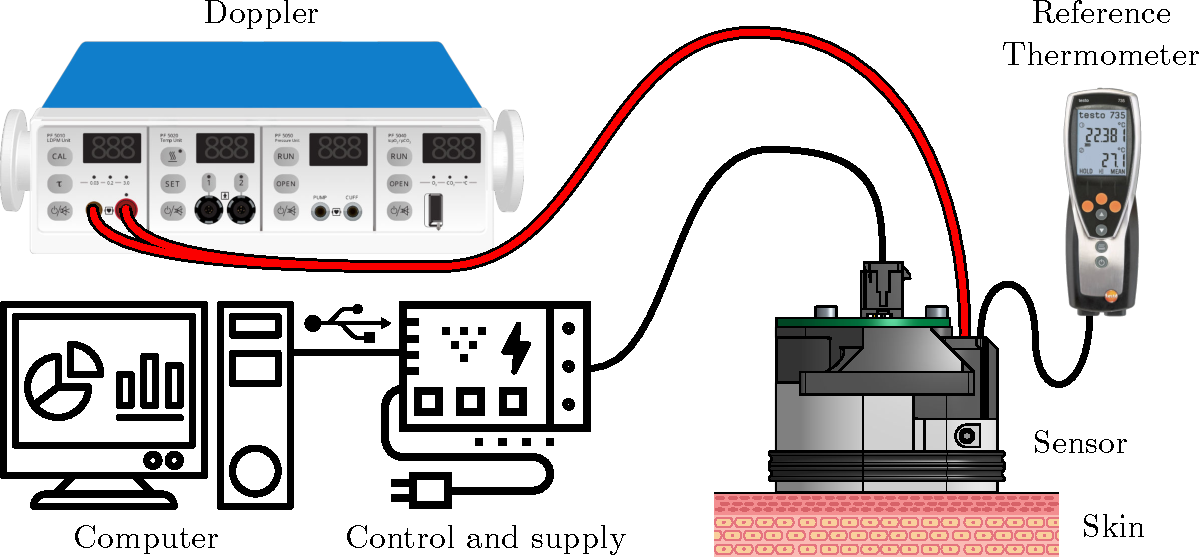
\includegraphics[width=\linewidth]{1_main_matter/tcco2_figures//global_schematic.pdf}
	\caption[General outline of the rate sensor and its peripherals.]{General outline of the rate sensor and its peripherals. See the text for further explanations.}\label{fig:tcco2:global_schematic}
\end{figure}

The sensor, designed to be placed against the subject's skin by means of a double-sided adhesive, is connected to three main apparatuses: \textit{(i)} a calibrated, reference thermometer (Testo 735, Testo, Germany) equipped with a type K thermocouple (110-4482, RS Pro, UK), \textit{(ii)} a Doppler perfusion monitor (Periflux 5000, Perimed, Sweden) equipped with a 407 probe, and \textit{(iii)} a control and supply block, consisting in a thermostat, a power supply unit, and a \gls{usb} to \gls{uart} converter, embedded in a 3D-printed case. For the sake of conciseness though, the control and supply block is only detailed in Appendix~\ref{app:tcco2_sm}, which also contains a thorough analysis of the safety issues that may arise when using this sensor. The sensor itself can be seen in great details in Figure \ref{fig:tcco2:explo_cut}. It consists in an aluminium (2017A) body, which serves as a support for the following elements: a \gls{co2} sensor, a heating resistive wire, a thermistor, a thermocouple, the Doppler probe, a \gls{pla} 3D-printed cover, and an interfacing \gls{pcb}. Complete drawings of the sensor's body are provided in Appendix~\ref{app:tcco2_sm}.

\begin{figure}
	\centering
	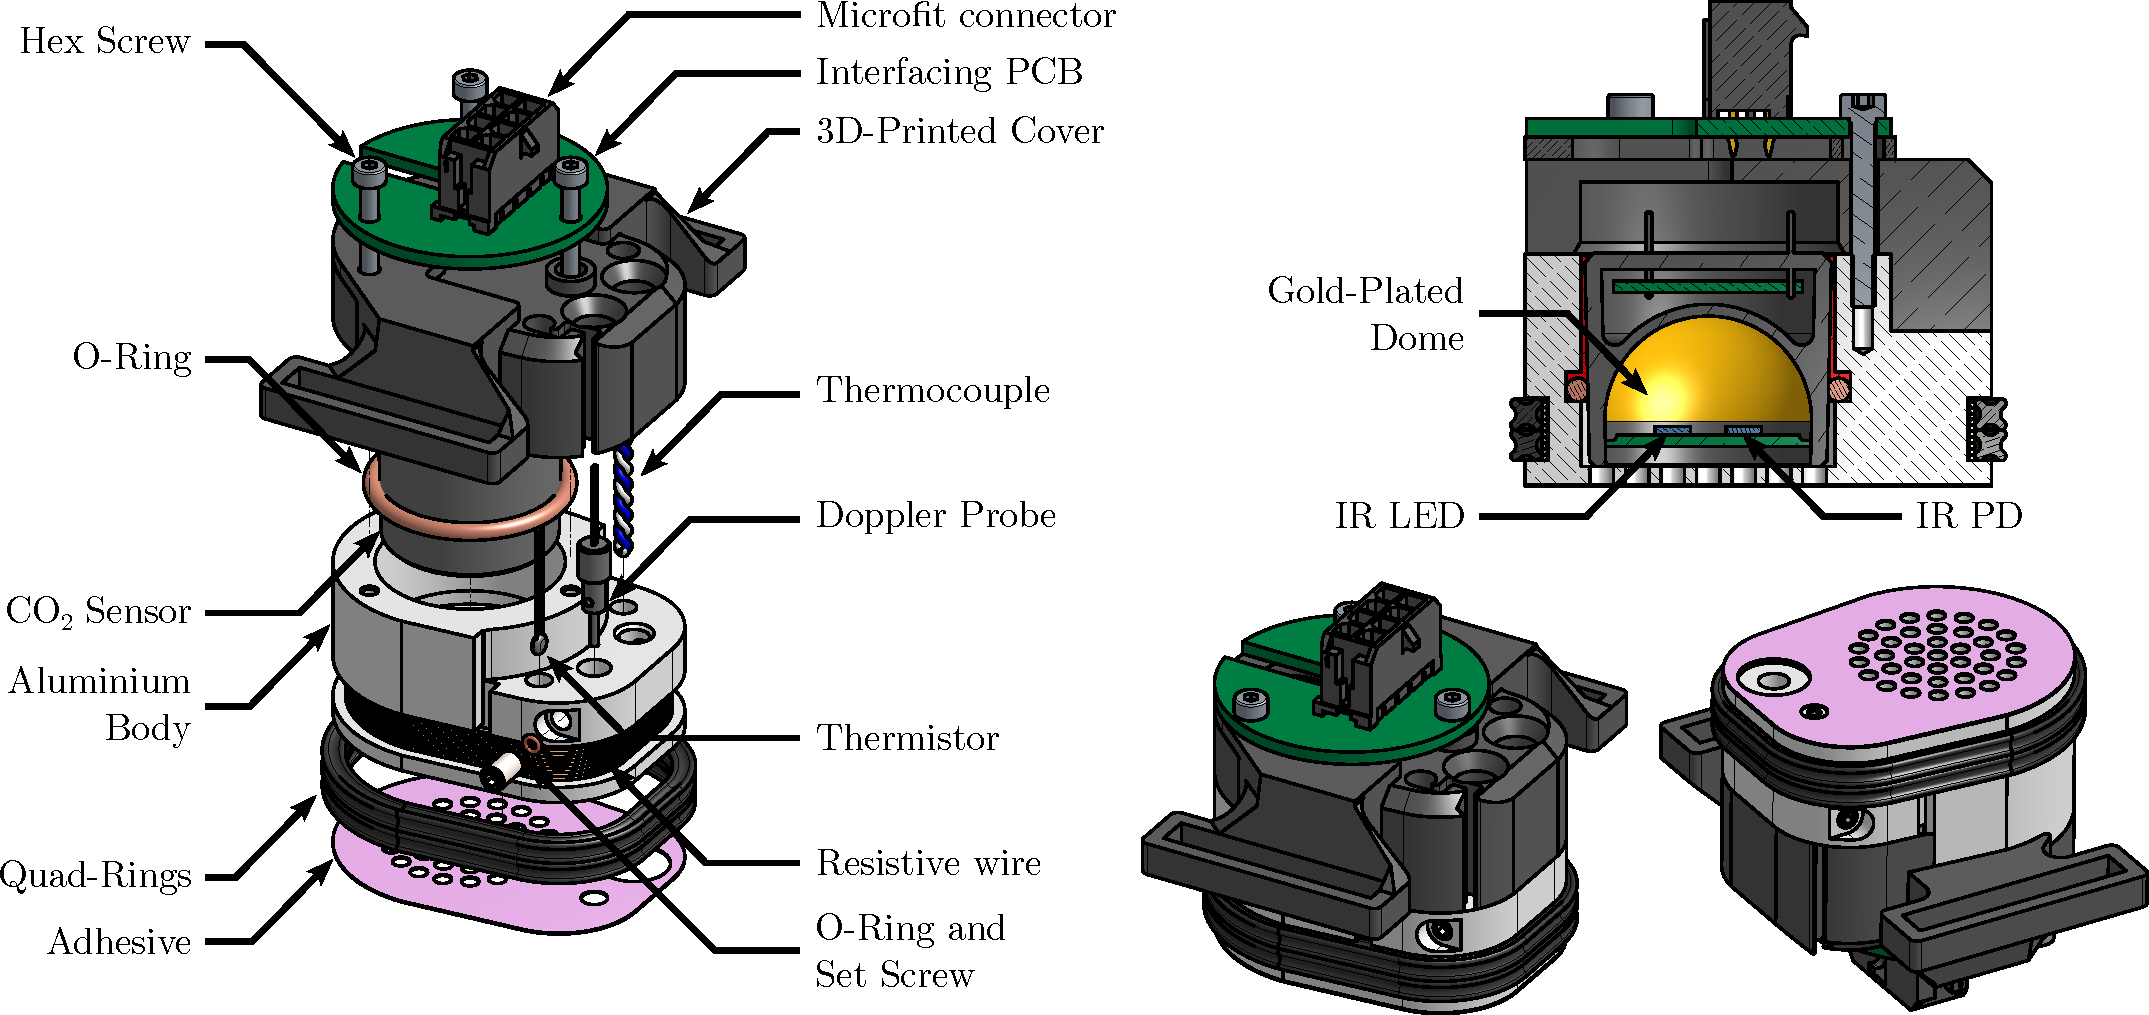
\includegraphics[width=\linewidth]{1_main_matter/tcco2_figures//explo_cut.pdf}
	\caption[Detailed views of the sensor.]{Detailed views of the sensor. \textbf{Left:} exploded view, detailing its different parts. \textbf{Top right:} cut view, showing the inner functioning principle of the \gls{co2} sensor. Note the epoxy resin sealing, in red. \textbf{Bottom right:} isometric views from above, and below, of the fully assembled sensor, illustrating the grid-shaped sensor's sole.}\label{fig:tcco2:explo_cut}
\end{figure}

\textbf{The \gls{co2} sensor} is a MinIR (ExplorIR - M5\%, CO2Meter, USA), an off-the-shelf, compact, \gls{ndir} \gls{co2} sensor, with a full range of 5\% and an accuracy of 70~ppm $\pm$5\% of reading at \gls{stp}---see Hodgkinson \etal{}\cite{hodgkinson2012rev} for further details on the operating principle of such sensors. Its internals---a pair of \gls{ir} \gls{led} and photodiode (PD) facing a spherical, gold-plated mirror---may be seen in the cut view of Figure \ref{fig:tcco2:explo_cut}. The \gls{pco2} inside the sensor was recorded with a sampling frequency of 2~Hz.

As the gas-tightness of the measuring chamber is a critical aspect of the sensor's operating principle---see Section \ref{subsect:tcco2:gas_tightness}---a two-stage sealing was implemented: \textit{(i)} a silicone-grease coated (515520, GEB, France), soft---60~Shore A hardness---silicone O-ring was placed between the aluminium body and the \gls{co2} sensor itself and \textit{(ii)} liquid epoxy resin (Résine Cristal, Gédéo, France) was cast in the remaining interstice between the latter two elements, illustrated in the cut view of Figure \ref{fig:tcco2:explo_cut} in vivid red.

\textbf{The thermoregulation} of the sensor is performed by means of a resistive wire for heating, coupled to a thermistor for temperature measurement and regulation. For verification purposes, an additional thermocouple was also added, as stated above. The heating wire consists in 2$\times$15 turns of 28~$\Omega$.m$^{-1}$, 0.15~mm in diameter, enamelled, resistive, constantan wire (Isotan, Thomsen), connected in parallel. The wire delivers a total heating power of 6.1~W under 12~V, and is coiled around the aluminium body, in a dedicated groove. The bottom of the groove is covered with a layer of 0.25~mm thermally conductive double sided tape (8810, 3M, USA) prior to coiling the wire, and the latter is finally covered with two nitrile quad rings, as can be seen in Figure \ref{fig:tcco2:explo_cut}. This covered layout prevents burns caused by direct contact with the heating wires. The thermistor (151-237, RS Pro, UK) and thermocouple were glued in two dedicated flat-bottom mounting holes which were pre-filled with a thermally conductive, electrically non-conductive, epoxy resin (8329TFM, MG Chemicals, Canada). Care was taken that \textit{(i)} the distance between the bottom of the mounting holes and the heating wire and \textit{(ii)} that between the sole of the sensor's body and the heating wire were equal, in order to ensure that the temperature measured by the thermistor and thermocouple is as close as possible to that of the skin.

\textbf{The Doppler probe} is housed in a dedicated hole, and can slide vertically, in such a way that it can be adjusted to outcrop the sole of the sensor, coming in direct contact with the skin. It holds in place by means of a cup-pointed, headless, set screw which compresses it radially via an O-ring, so as not to damage the probe. The raw Doppler perfusion signal---originally sampled at 62.5~Hz---was downsampled to 0.625~Hz and low-pass filtered using a tenth-order Butterworth filter prior to further analysis---see Section \ref{subsect:tcco2:subcut_bf}.

\textbf{The 3D-printed cover and interfacing \gls{pcb}} were added for usability purposes: the 3D-printed \gls{pla} cover allows to attach a strap (HTH 833 with H83 hooks, Velcro, UK) to the sensor in order to maintain it against a subject's skin, as illustrated in Figure \ref{fig:tcco2:photo_pos}, Right, while the interfacing \gls{pcb} gathers the four \gls{uart} pins from the \gls{co2} sensor, the two ends of the thermistor, and those of the heating wire into a single eight-pins Microfit connector (0430450812, Molex, USA).

\begin{figure}
	\centering
	\includegraphics{1_main_matter/tcco2_figures/tikz/out/photo_pos_comp.pdf}
	\caption[Location and photo of the sensor.]{\textbf{Left:} outline of the sensors used in this study, and their location. \textbf{Right:} a picture of the sensor with its connection cable assembly and strap, attached on a wrist.}\label{fig:tcco2:photo_pos}
\end{figure}

\textbf{The adhesive} itself consists in a disposable laser-cut, double-sided, clinical-grade tape (1567, 3M, USA). For ease of application, a special tooling was developed to accurately align the sensor and the adhesive together---see Appendix~\ref{app:tcco2_sm}.

\subsubsection{Reference \texorpdfstring{\gls{ptco2}}{tcpCO2} Monitor}

In addition to the above-detailed custom-made sensor, a clinical-grade \gls{ptco2} monitor (TCM4, Radiometer, Denmark) was also used on the upper deltoid---one of the recommended sites for \gls{ptco2} monitoring\cite{vsign_brochure}---yielding a continuous reference \gls{ptco2} reading. The \gls{ptco2} sensor itself (tc Sensor 54) was affixed to the skin using an appropriate attachment ring and contact gel, and it was re-membraned and re-calibrated when needed, as per the manufacturer's guidelines. All the accessories used to this end were Radiometer's\cite{radiometer_combim}.

\subsubsection{Sensors Positioning}

The different sensors and measurement sites chosen in the study are illustrated in Figure \ref{fig:tcco2:photo_pos}, Left. All sensors were placed on the subject's left arm: the reference \gls{ptco2} monitor was placed on the upper deltoid, as mentioned above, while two custom rate sensors were positioned as follows. The first one was equipped with the Doppler probe, and was attached on the distal side of the upper arm, immediately below the deltoid, at the junction point between the upper part of the biceps, the lower end of the deltoid, and the triceps. The second rate sensor was placed on the dorsal side of the wrist, and did not include a Doppler probe. Both sensors were affixed to the subject's skin by means of the above-mentioned double-sided adhesive, and secured in place with a Velcro strap. Additionally, the subject's arm laid comfortably onto an arm gutter so that it remained still and relaxed for the whole duration of the experiments.

\subsection{Methods}\label{sect:methods}

\subsubsection{Measured Metrics}

\paragraph{Skin \texorpdfstring{\gls{co2}}{CO2} Conductivity and Exhalation Rate}\label{subsect:tcco2:co2_conductivity}\mbox{}\\

The rate of diffusion---\aka{} the exhalation rate---of \gls{co2} through the skin per unit of area---hereafter noted $Q$, of dimension L$^3$~L$^{-2}$~T$^{-1}$---can be measured by affixing to the skin a cup-like device, which entraps the skin-exhaled \gls{co2}. In this situation, the \gls{co2} diffusion through the skin can be modelled as already presented in Figure \ref{fig:tcco2:diffusion_model} and Section~\ref{sect:tcco2:modelling_tc_sensing}. Briefly, the skin is considered as a \gls{co2}-permeable membrane of thickness $w$ and diffusivity $D$ towards \gls{co2} (unit of m$^2$.s$^{-1}$). The partial \gls{co2} pressure inside the sub-cutaneous tissues and inner chamber are \gls{ptco2} and \gls{pseco2}, respectively, and the sensor area in contact with the skin is $S_\text{Se}$, while its equivalent height and volume are $h_\text{Se}$ and $V_\text{Se}$. It can be shown under certain hypotheses---see Section~\ref{sect:tcco2:modelling_tc_sensing}---that
\begin{equation}\label{eq:tcco2:equa_diff_comp}
	\frac{d \text{\gls{pseco2}}}{dt} = \frac{D}{w \cdot h_\text{Se}} \cdot \left( \text{\gls{ptco2}} - \text{\gls{pseco2}} \right)
\end{equation}
leading to a first-order behaviour for \gls{pseco2}, given by
\begin{equation}\label{eq:tcco2:pseco2_full}
	\text{\gls{pseco2}}(t) = \text{\gls{ptco2}} \cdot \left( 1 - e^{ -\frac{t}{\tau} } \right) + \text{\gls{pseco2}}(t=0) \cdot e^{ -\frac{t}{\tau}}, \quad \text{with } \tau = \frac{h_\text{Se} \cdot w}{D}
\end{equation}
and $Q$ is then equal to
\begin{equation}\label{eq:tcco2:q_def}
	Q(t) = \frac{D}{w \cdot \text{p}_0}\cdot \left(\text{\gls{ptco2}} - \text{\gls{pseco2}}(t=0)\right) \cdot e^{ -\frac{t}{\tau}}
\end{equation}
wherein p$_0$ is the total atmospheric pressure at measurement site. However, since $Q$ depends on both the ambient level of \gls{co2}---\textit{via} \gls{pseco2}$(t=0)$---and the subject's capnia---\textit{via} \gls{ptco2}---we introduced the skin \emph{conductivity}---from the thermodynamic or electrical analogy---expressed in m.s$^{-1}$, and defined as
\begin{equation}\label{eq:tcco2:k_def}
	\boxed{K = \frac{D}{w}} = \frac{P_0 \cdot Q(t=0)}{\text{\gls{ptco2}} - \text{\gls{pseco2}}(t=0)}
\end{equation}

Contrary to $Q$, $K$ is an intrinsic property of the skin and is independent of the \gls{ptco2} / \gls{pseco2} gradient. Additionally, deriving Equation \ref{eq:tcco2:pseco2_full} and evaluating it at $t=0$ yield
\begin{equation}\label{eq:tcco2:k_effective_calc}
	K = \frac{h_\text{Se}}{\text{\gls{ptco2}} - \text{\gls{pseco2}}(t=0)} \cdot \frac{d\text{\gls{pseco2}}}{dt} \biggr\rvert_{t=0}
\end{equation}

In practice, $K$ was thus measured as follows, choosing arbitrarily $t=0$ at each temperature change:
\begin{itemize}
	\item[--] $h_\text{Se}$ is known by dividing $V_\text{Se}$ by $S_\text{Se}$. The latter is known by construction of the sensor's aluminium body, while $V_\text{Se}$ was estimated by filling a clone of the sensor with a low viscosity fluid---pure ethanol---and weighting it.
	\item[--] the subject's \gls{ptco2} was measured using the above-mentioned reference medical grade monitor. The extraction of a single \gls{ptco2} reading for each temperature set-point is detailed in Appendix~\ref{app:tcco2_sm}.
	\item[--] \gls{pseco2}$(t=0)$ could be measured with a simple reading of the \gls{co2} sensor.
	\item[--] $\frac{d\text{\gls{pseco2}}}{dt} \biggr\rvert_{t=0}$ was estimated by fitting a linear regression to the measured \gls{pseco2}. The latter regression was performed on the \gls{pseco2} data starting 3~min after a temperature change---to allow for temperature homogenisation of the different inner parts of the sensor---and until 18~min after, for a total of 15~min of data. This duration was chosen following a preliminary study performed on ten subjects, which yielded $R^2$ regression scores above 0.95 for a regression duration above 700~s (about 12~min).
\end{itemize}

In summary, \textbf{the diffusion of $\mathbf{CO_2}$ through the skin was quantified by the skin $\mathbf{CO_2}$ conductivity $\boldsymbol{K}$}, which was measured at five different temperatures, each temperature corresponding to a 18~min measurement window for a total of 90~min of acquisition per subject, as detailed in Section \ref{subsect:tcco2:protocol}, below. Additionally, Equation \ref{eq:tcco2:k_def} was used to compute the corresponding equivalent $Q(t=0)$ with \gls{pseco2}$(t=0)\approx 0$---\ie{} the skin \gls{co2} exhalation rate in free air as commonly referred to in the literature. Of note, this $Q(t=0)$ was \textbf{not} observed in practice, since the sensor was left in place---and thus \gls{pseco2}$(t=0)\neq 0$ for most temperatures. For the sake of conciseness, in the remainder of this chapter, the letter $Q$ alone or the mention of \enquote{skin \gls{co2} exhalation rate} without further indications always designate the above-mentioned $Q(t=0)$. Finally, it should be noted that these $Q$ values were derived mainly as a means of comparison with the existing literature, and that the actual statistical analyses were performed on $K$---see Section \ref{subsect:tcco2:data_anal}.

\paragraph{Skin Blood Flow}\label{subsect:tcco2:subcut_bf}\mbox{}\\

The skin blood flow---\aka{} (sub)cutaneous micro-circulation or perfusion---was measured using \gls{ldf}, and expressed in \gls{punit}, a dimensionless arbitrary unit that reflects both the amount and the speed of moving elements---mainly erythrocytes---seen by the Doppler probe\cite{bonner1990}. When the skin temperature rises, perfusion increases, a phenomenon known as heat-triggered---or thermal---reactive hyperaemia\cite{minson2010}, whose dynamics is illustrated in Figure \ref{fig:tcco2:doppler_principle}, Left. The respective durations of phases \Circled{1}--\Circled{3} were not specified in abscissa since they may vary markedly depending on the heating rate and temperature\cite{magerl1996, delpozzi2016}. To give the reader an order of magnitude, phase \Circled{1} usually lasts a few minutes, phase \Circled{2} from 5 up to 10~min, and phase \Circled{3} from 30 up to 60~min\cite{cracowski2006, frantz2012, minson2001, minson2010, roustit2012}.

\begin{figure}
	\centering
	\includegraphics[width=\linewidth]{1_main_matter/tcco2_figures/tikz/out/doppler_principle.pdf}
	\caption[Skin perfusion response to local heating.]{\textbf{Left:} typical skin perfusion response to local heating, schematised from different sources\cite{cracowski2006, frantz2012, minson2001, minson2010, roustit2012}. If we suppose the heat stress to be applied at time origin, three phases are usually observed: \Circled{1} an onset lag corresponding to \emph{(i)} the heating time required by the sensor to reach its set-point temperature and \emph{(ii)} the time taken by the inner skin layers to reach this temperature and trigger the axon-mediated hyperaemia. \Circled{2} the axon-mediated hyperaemia which rises quickly and then fades away. \Circled{3} the nitric-oxide mediated hyperaemia, whose onset is slower and which slowly fades away if the temperature set-point is not too elevated. \textbf{Right:} perfusion and skin temperature as a function of time as measured at the arm of a test subject.}\label{fig:tcco2:doppler_principle}
\end{figure}

Such a behaviour calls for some kind of data processing to yield a single representative perfusion metric for the initial bump, after-bump nadir, and final plateau. In this study, SkBF$_{90}$(T) was defined as the 90$^\text{th}$ percentile of the measured skin blood flow---SkBF---on a 18~min window at temperature T. This choice was made following preliminary measurements at the arm, an example of which is plotted in Figure \ref{fig:tcco2:doppler_principle}, Right. The latter clearly exhibits five perfusion plateaux corresponding to the five temperature set points, and one can also distinguish a small initial bump at the onset of a new temperature, which is especially visible at 35, 38 and 41{\degree}C. Due to \textit{(i)} the high variability exhibited by the measured perfusion, especially at high temperature, \textit{(ii)} the fact that the nitric-oxide phase can take up to 30--40~min to establish\cite{barcroft1943, taylor1984, minson2001, frantz2012, delpozzi2016}, and \textit{(iii)} the fact that each temperature window lasts 18~min, it seemed a good strategy to choose a metric which was more robust than the mean---\eg{} the n-th percentile---and focused on the very end of the observation window. In this regard, SkBF$_{90}$(T) seemed to meet the latter requirements and was therefore chosen as perfusion metric. It was additionally normalised by the maximal perfusion measured on a given subject---\ie{} the SkBF$_{90}$ value measured at 44{\degree}C. Finally, the \gls{ldf} metric used throughout this study is thus
\begin{equation}
	\boxed{
		\mathrm{nSkBF_{90}(T)} = \frac{\mathrm{SkBF_{90}(T)}}{\mathrm{SkBF_{90}(44{\degree}C)}}
	}
\end{equation}

\subsubsection{Protocol Design}\label{subsect:tcco2:protocol}

The clinical study was interventional, monocentric, and involved 40 healthy human subjects. Inclusion criteria were an age between 18 and 80, and having given a free and informed consent. Exclusion criteria were the presence of cutaneous lesions at the measurement sites or skin conditions such as dermatitis or psoriasis, and taking vasodilator therapy. The research was approved by the local ethics committee (Comité de protection des personnes Sud-Méditerrannée II, IDRCB ref.: 2020-A02185-38), registered on Clinical Trials (\href{https://web.archive.org/web/20230224073221/https://clinicaltrials.gov/ct2/show/NCT05637138}{NCT05637138}), and it was carried out in accordance with the declaration of Helsinki.

After a preliminary visit during which the subjects were informed of the study modalities and gave consent, all measurements were performed during a single visit, during which the subjects were seated. This visit began with a visual inspection of the measurement sites for detection of cutaneous lesions. The sites were then shaved if needed for a good adhesion of the sensors, using an electric trimmer in order to avoid skin inflammation. The skin was then degreased and cleaned using isopropyl alcohol, and the three above-mentioned sensors were attached to their respective measurement sites. These preliminary steps also allowed for subject acclimation and lasted about 5~min. The measurement itself then began, consisting of five 18~min periods, corresponding to five temperatures for the two rate sensors: \gls{nh}, 35, 38, 41, and 44{\degree}C. At the end of the 90~min measurement period, the sensors were gently peeled off, and the skin was cleaned again. All \gls{ptco2} and \gls{pseco2} data were recorded on computers for future analysis, and the room temperature was also recorded using a calibrated thermometer (Testo 735, Testo, Germany).

\subsection{Data Analysis}\label{subsect:tcco2:data_anal}

The data analysis workflow is summarised in Figure \ref{fig:tcco2:data_analysis}. Raw data were collected for all 40 subjects at five different temperatures and three metrics were extracted for each i-th subject / temperature pair: $K$ at the arm and wrist, and nSkBF$_{90}$ at the arm only. For each of those metrics, an \gls{anova} was performed across all subjects to determine whether their mean values differed significantly between two temperatures. If the \gls{anova} residuals did not significantly differ from a normal distribution---according to Shapiro-Wilk testing---and if the hypothesis of variance equality between the temperature groups was also verified---according to Bartlett testing---a Tukey post-hoc HSD test was then performed. Otherwise, a Kruskal-Wallis test followed by a series of Mann-Whitney U-tests were performed. Additionally, Pearson and Spearman correlation tests were also carried out to study the influence of temperature on the three afore-mentioned metrics (not represented in Figure \ref{fig:tcco2:data_analysis}). When applicable, all tests were two-sided and a 5\% alpha risk was chosen as significance threshold.

\begin{figure}
	\centering
	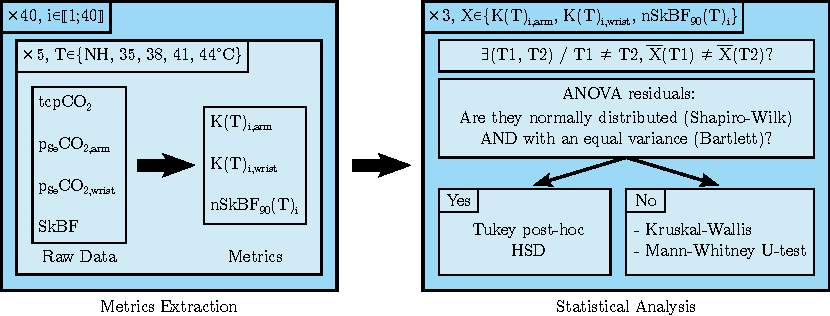
\includegraphics{1_main_matter/tcco2_figures/data_analysis.pdf}
	\caption[Graphical representation of the data analysis workflow.]{Graphical representation of the data analysis workflow, see the text for further details.}\label{fig:tcco2:data_analysis}
\end{figure}

\subsection{Results}\label{sect:tcco2:results}

\subsubsection{Demographics and Temperatures}

The forty subjects consisted in 24 men and 16 women, aged between 20 and 61 years (mean / median / \gls{sd}: 40 / 39 / 13 years). The laboratory temperature was in the 20.1--22.7{\degree}C range for the whole duration of the experiments (mean / median / \gls{sd}: 21.3 / 21.2 / 0.7{\degree}C). The skin temperature during the non-heated 18~min phase was measured twice, at 10 and 18~min after sensor application, and these two measurements were averaged to yield a single temperature value per subject. The latter was in the 27.1--31.8{\degree}C range (mean / median / \gls{sd}: 29.3 / 29.2 / 1.2{\degree}C) at the arm, and in the 24.7--33.1{\degree}C range (mean / median / \gls{sd}: 28.6 / 28.5 / 1.7{\degree}C) at the wrist.

\subsubsection{Skin \texorpdfstring{\gls{co2}}{CO2} Conductivity}\label{subsect:tcco2:results:ks}

The linear regressions leading to $K$ values---see Section \ref{subsect:tcco2:co2_conductivity}---yielded excellent regression coefficients, with average $R^2$ values of 0.98 and 0.96 at the arm and wrist, respectively. The resulting skin conductivities are summarised in Figure \ref{fig:tcco2:ks_boxplot}, and show a sharp tendency to increase with an increasing skin temperature. Interestingly, the five upper outlying values at the arm---at all temperatures---and the four upper and lower outlying values at the wrist---in the 35--44{\degree}C range---belonged each time to a single subject, who exhibited an especially high, or low skin conductivity. However, these two latter subjects were not one and the same person at the arm and at the wrist. The dispersion of skin conductivity values is also glaring with max / min ratios for a given skin temperature / location pair in the 2.9--9.0 range.

\begin{figure}
	\centering
	\includegraphics[width=\linewidth]{1_main_matter/tcco2_figures/tikz/out/ks_boxplot.pdf}
	\caption[Skin conductivities at the arm and wrist (box plots).]{Skin conductivities at the arm and wrist. Each black mark corresponds to a subject / temperature pair, the red circles and texts indicate mean values, and some horizontal jitter was added to the black marks for legibility. The whiskers extend at most to 1.5 times the interquartile range, and descriptive statistics---range, and SD---are provided in Appendix~\ref{app:tcco2_sm}. These properties are shared by the three box plots of the present section.}\label{fig:tcco2:ks_boxplot}
\end{figure}

A normalisation of the variable $K$---using the change of variable $K\mapsto\sqrt{K}$---was carried out prior to the \gls{anova}, resulting in the Shapiro-Wilk and Bartlett tests to be passed (all p-values above 0.05). The \gls{anova} was significant (p-value below $10^{-15}$) and the results of the following Tukey post-hoc HSD test are detailed in Table \ref{table:tcco2:stats_ks}. The apparent increase in $K$ with an increasing skin temperature seen in Figure \ref{fig:tcco2:ks_boxplot} is hereby confirmed, with significantly different mean $K$ values for most temperature differences except the closest ones---\ie{} for the 35/38, 38/41 and 41/44{\degree}C pairs.

\def\arraystretch{1.25}
\begin{table}
	\centering
	\small
	\begin{minipage}{.5\linewidth}
		\centering
		\begin{tabular}{c|c|c|c|c}
			{Arm} & N.H. & 35{\degree}C & 38{\degree}C & 41{\degree}C \\ \hline
			35{\degree}C & $<10^{-6}\dagger$ & - & - & -\\
			38{\degree}C & $<10^{-6}\dagger$ & 0.72 & - & -\\
			41{\degree}C & $<10^{-6}\dagger$ & 0.05$\dagger$ & 0.54 & -\\
			44{\degree}C & $<10^{-6}\dagger$ & $<10^{-3}\dagger$ & 0.01$\dagger$ & 0.44
		\end{tabular}	
	\end{minipage}%
	\begin{minipage}{.5\linewidth}
		\centering
		\begin{tabular}{c|c|c|c|c}
			{Wrist} & N.H. & 35{\degree}C & 38{\degree}C & 41{\degree}C \\ \hline
			35{\degree}C & $<10^{-6}\dagger$ & - & - & -\\
			38{\degree}C & $<10^{-6}\dagger$ & 0.35 & - & -\\
			41{\degree}C & $<10^{-6}\dagger$ & $<10^{-3}\dagger$ & 0.14 & -\\
			44{\degree}C & $<10^{-6}\dagger$ & $<10^{-6}\dagger$ & $<10^{-3}\dagger$ & 0.73
		\end{tabular}	
	\end{minipage}
	\caption[p-values for the Tukey HSD post-hoc test for differences of the mean $K$ at different temperatures.]{p-values for the Tukey HSD post-hoc test for differences of the mean $K$ at different temperatures. Values with a $\dagger$ are considered significant with a risk $\alpha$=0.05. (Only the lower-left parts of the tables are filled-in for the sake of clarity.)}\label{table:tcco2:stats_ks}
\end{table}

Pearson and Spearman correlations were both significant (p-values below $10^{-15}$) with correlation coefficients of 0.60 and 0.59 at the arm, respectively, and 0.66 and 0.67 at the wrist. These coefficients indicate a moderate positive influence of the skin temperature on its diffusivity towards \gls{co2}.

\subsubsection{Skin \texorpdfstring{\gls{co2}}{CO2} Exhalation Rate}

In order to provide a more accessible parameter than $K$ to the reader, as well as to allow direct comparison with existing literature, equivalent initial exhalation rates $Q(t=0)$ were also computed using Equation \ref{eq:tcco2:k_def}. The resulting values are presented in Table \ref{table:tcco2:qs_values}.

\def\arraystretch{1.25}
\begin{table}
	\centering
	\begin{minipage}{.5\linewidth}
		\centering
		\begin{tabular}{c|c|c|c}
			{Arm} & Mean & Range & S.D. \\ \hline
			N.H. & 80.4 & 25.1--191.7 & 40.3\\
			35{\degree}C & 130.3 & 52.4--227.4 & 43.5 \\
			38{\degree}C & 142.7 & 63.0--248.1 & 41.4 \\
			41{\degree}C & 159.9 & 81.9--280.2 & 42.8 \\
			44{\degree}C & 177.5 & 104.6--288.4 & 42.5
		\end{tabular}	
	\end{minipage}%
	\begin{minipage}{.5\linewidth}
		\centering
		\begin{tabular}{c|c|c|c}
			{Wrist} & Mean & Range & S.D. \\ \hline
			N.H. & 58.7 & 24.2--141.1 & 22.7 \\
			35{\degree}C & 100.9 & 27.7--220.6 & 38.3 \\
			38{\degree}C & 118.2 & 27.1--248.0 & 42.8 \\
			41{\degree}C & 141.8 & 36.0--282.1 & 47.2 \\
			44{\degree}C & 162.3 & 46.5--300.0 & 45.9
		\end{tabular}	
	\end{minipage}
	\caption{$Q(t=0)$ values, as computed using Equation \ref{eq:tcco2:k_def}, expressed in cm$^3$.m$^{-2}$.h$^{-1}$.}\label{table:tcco2:qs_values}
\end{table}

Although our results tend to indicate a higher \gls{co2} exhalation rate at the upper arm than at the wrist---a \gls{manova} was performed considering the measurement site as an independent variable and the five $Q_T$ as dependent variables, and yielded a p-value of 0.01 using Pillai's trace---the size of this effect is moderate, especially in view of the wide $Q$ dispersion.

\subsubsection{Laser Doppler Flowmetry}

nSkBF$_{90}$ values were computed as described in Section \ref{subsect:tcco2:subcut_bf}, and are presented in Figure \ref{fig:tcco2:nskbf_boxplot}. Skin perfusion exhibits a strong increase with temperature, with a tenfold multiplication between the \gls{nh} basal state and the maximum vasodilation 44{\degree}C stage. In particular, a mild heating to a temperature of 38{\degree}C already entails a fourfold increase in perfusion. As was the case for skin conductivity, the dispersion of the nSkBF$_{90}$ values is also considerable, with max / min ratios for a given temperature in the 2.2--9.7 range.

\begin{figure}
	\centering
	\includegraphics{1_main_matter/tcco2_figures/tikz/out/nskbf_boxplot.pdf}
	\caption[Measured nSkBF$_{90}$ at the arm.]{Measured nSkBF$_{90}$ at the arm. Note that since nSkBF$_{90}$ is normalised with respect to SkBF$_{90}$ at 44{\degree}C, all subjects merge into a single unitary value at this temperature. Each black mark corresponds to a subject / temperature pair, the red circles and texts indicate mean values, and the red curve is a least square sigmoid fit. Contrary to Figure \ref{fig:tcco2:ks_boxplot}, no horizontal jitter was added to the data, and the dispersion observed in the 27--32{\degree}C range corresponds to the inter-subject variability in non-heated skin temperatures.}\label{fig:tcco2:nskbf_boxplot}
\end{figure}

Regarding statistical analyses, the normality and variance homogeneity hypotheses could not be verified regardless of the changes of variable performed. A Kruskal-Wallis test was thus conducted, followed by a series of Mann-Whitney U-tests, all of which proved significant (all p-values below $10^{-10}$).

Pearson and Spearman correlations were both significant (p-values below $10^{-15}$) with correlation coefficients of 0.90 and 0.96, respectively. These coefficients indicate a strong positive influence of the skin temperature on its perfusion. The fact that Pearson's correlation is below Spearman's is not surprising since the relationship between skin temperature and nSkBF$_{90}$ is strongly non-linear, as emphasised by the sigmoid fit performed in Figure \ref{fig:tcco2:nskbf_boxplot}.

\subsection{Discussion}\label{sect:discussion}

The main objectives of this research were to ascertain the influence of skin temperature on \textit{(i)} its permeability towards \gls{co2}---through the study of the skin \gls{co2} conductivity $K$, and exhalation rate $Q$---and \textit{(ii)} the skin blood flow---through nSkBF$_{90}$.

\subsubsection{Sensor Design}

\paragraph{Skin Contact Surface}\label{subsect:tcco2:skin_surface}\makebox{}\\

Although the sensor's aluminium body was precisely machined following the drawing given in Appendix~\ref{app:tcco2_sm}, the exact surface area in contact with the skin that participates in gaseous exchanges may slightly vary from one subject to another. Indeed, at each hole of the sensor's sole, the skin forms a small dome, whose convexity is essentially a function of the mechanical properties of the skin. Yet, those mechanical properties are sex-, moisture-, age-, and temperature-dependant\cite{salter1993, held2018}, thereby introducing small intra- or inter-subject variations in skin contact surface area. Since this area is used to calculate $K$ through $S_{Se}$---see Section \ref{subsect:tcco2:co2_conductivity}---the latter is in turn influenced by these small variations.

While this would likely not change the conclusions of the present study given the order of magnitude of the above-described phenomenon reported in the literature, \mfrin{}future research could look into replacing the grid-shaped sole that we used by a thin metal mesh, or a metallic foam. These two techniques were for instance implemented by Eletr, McIlroy, Hansen \etal{}\cite{eletr1978, mcilroy1978, hansen1980}. However, it must be emphasised that the shape of the sole of a thermally-regulated transcutaneous exhalation rate sensor is essentially a compromise between: \emph{(i)} the degree of perforation or porosity of the surface, which should be as high as possible to ensure a large diffusion surface, and \emph{(ii)} heat transfer considerations, which call for a plain, dense, surface, with a minimum number of holes, to ensure temperature homogeneity of the skin. Additionally, while the use of a wire mesh, or metallic foam reduces the above-mentioned \enquote{dome effect}, it also makes the surface estimation more tedious. Therefore, this aspect of the sensor design should be further investigated to find a satisfactory technical solution which addresses the above concerns.

\paragraph{\texorpdfstring{\gls{co2}}{CO2} Sensor Choice}\makebox{}\\

The choice of the selected \gls{ndir} \gls{co2} sensor was mainly motivated by its compact form factor and ease of implementation. Additionally, the 5\% range was especially adapted for \gls{co2} diffusion rate measurements. Indeed, \gls{ptco2} in healthy subjects is typically in the 35--45~mmHg range\cite{rithalia1984}, corresponding to 4.6--5.2\% of \gls{co2}. Since the \gls{co2} diffusion rate measurements taking place in the present study were only limited to the first moments of \gls{co2} diffusion from the skin into the sensor---see Section \ref{subsect:tcco2:co2_conductivity}---measured \gls{co2} fraction values stayed below 1--2\%. The 5\% range was thus adapted to our need.

\paragraph{Gas Tightness}\label{subsect:tcco2:gas_tightness}\makebox{}\\

As mentioned in Section~\ref{subsect:tcco2:mat_sensor}, the gas tightness of the sensor's chamber with respect to ambient air was of paramount importance for the success of the study. Indeed, any leak of inner-chamber \gls{co2} towards the outer air would subtract from the measured rate of exhalation of \gls{co2} through the skin, and thus impair the resulting $K$ values. During the sensor's design, gas tightness was assessed by sticking the sensor onto a glass plate using the same adhesive as for the human-testing part of the study. The so-obtained glass plate / sensor pair was then put inside a chamber that was successively filled with a 2.5\% \gls{co2} / \gls{n2} mixture and fresh air. The resulting measurements are presented in Figure \ref{fig:tcco2:gas_tightness}, Centre, and clearly demonstrate that the greased O-ring alone was not gas tight, while the epoxy sealing was. The left part of Figure \ref{fig:tcco2:gas_tightness} also illustrates in a cut view how the epoxy seal complements the O-ring. In practice, the grease-coated O-ring acts as a resin-proof sealing that prevents the resin from flowing inside the sensor's chamber during its casting process.

\begin{figure}
	\centering
	\includegraphics[width=0.99\linewidth]{1_main_matter/tcco2_figures/tikz/out/fig_sealing.pdf}
	\caption[Sensor sealing analysis.]{\textbf{Left:} close up of the section view of Figure \ref{fig:tcco2:explo_cut}, showing the two key elements of the gas tight seal: a grease-coated O-ring, and cast epoxy resin (in red). \textbf{Centre:} a sealing test comparing the greased O-ring alone with the greased O-ring and the cast epoxy resin. This test clearly indicates that the greased O-ring alone does not accomplish gas tightness, whereas the cast epoxy resin does. \textbf{Right:} sensor sensibility towards humidity, showing the onset of condensation onto the gold-plated dome. This condensation drastically reduces the quantity of light reaching the detector, effectively blinding it, which is interpreted as an exceedingly elevated \gls{co2} concentration.}\label{fig:tcco2:gas_tightness}
\end{figure}

This gas tightness allows \gls{co2} to accumulate into the sensor chamber until an equilibrium is reached between the subcutaneous tissues and the sensor's chamber---\ie{} until \gls{pseco2}~=~\gls{ptco2}. While this equilibrium---although it would take several hours given the respective order of magnitudes of $Q$ and $h_\text{Se}$---and the associated \gls{co2} diffusion process are at the very heart of this study, another undesirable chemical species will also accumulate into the sensor's chamber due to the combined action of diffusion and sweating: water vapour.

While the influence of water vapour on \gls{ndir} \gls{co2} measurements due to the infrared absorbance of water vapour is expected to be negligible given the large gap between \gls{co2} and water vapour infrared absorption bands\cite{se_ndir_co2}, the onset of condensation onto the reflective part of the sensor---namely the gold-coated reflective dome---can still be an issue. Indeed, the formation of micro-droplets of condensing water onto the latter dome would drastically reduce its reflectance, fooling the sensor into believing that a large amount of \gls{co2} is present inside the sensor's chamber---a well-known issue in \gls{ndir} sensing\cite{fietzek2014, wang2018}. In order to study the influence of condensing humidity levels onto the sensor used in the present research, two experiments were carried out whose outcomes are presented in Figure~\ref{fig:tcco2:gas_tightness}, Right. The first experiment consisted in placing the sensor on a human thigh at increasing temperatures and waiting for condensation to occur, which happened after 30~min at 44{\degree}C. The second experiment consisted in bubbling ambient air (20{\degree}C) through pumice stone inside a hot water bath, yielding water-saturated hot air (40{\degree}C), which was then flowed onto the un-heated sensor. Even in these unfavourable conditions---\ie{} a cold sensor and water-saturated hot air---it took about 20~min to detect the onset of condensation on \gls{co2} measurements. Given that the latter onset was particularly sudden and visible on \gls{pseco2} in both experiments, the influence of water vapour condensation on this study was deemed negligible. Indeed, it would be easily detected---were it to happen while measuring a given subject---and the corresponding measurement would be discarded, something which did not happen in practice.

Finally, the reader should bear in mind that the gas tightness of the sensor and the accumulation of humidity underneath it both create a condition called \emph{skin occlusion}. This occlusion, while out of the scope of this section, has been studied by several authors\cite{frame1972, king1978, faergemann1983}, who reported much higher \gls{co2} exhalation rates for long-term---\ie{} days---occluded skin, as compared to its basal state. \mfrin{}This phenomenon was not investigated in the present study due to the long time scale that it involves, but further research on this topic would be welcome.

\paragraph{Sensors Positioning}\label{sect:tcco2:frontiers:sensor_pos}\makebox{}\\

To our knowledge, only three studies compared the influence of the measurement site on the transcutaneous \gls{co2} diffusion rate in humans: that of Schulze on twelve subjects\cite[Table~16]{schulze1943}, that of Adamczyk \etal{}\cite{adamczyk1966} on one subject, and that of Levshankov \etal{}\cite{levshankov1983} on an unspecified number of subjects. The results of the latter two authors are summarised in Figure \ref{fig:tcco2:positioning}---Schulze indications were difficult to interpret and were thus not illustrated.

\begin{figure}
	\centering
	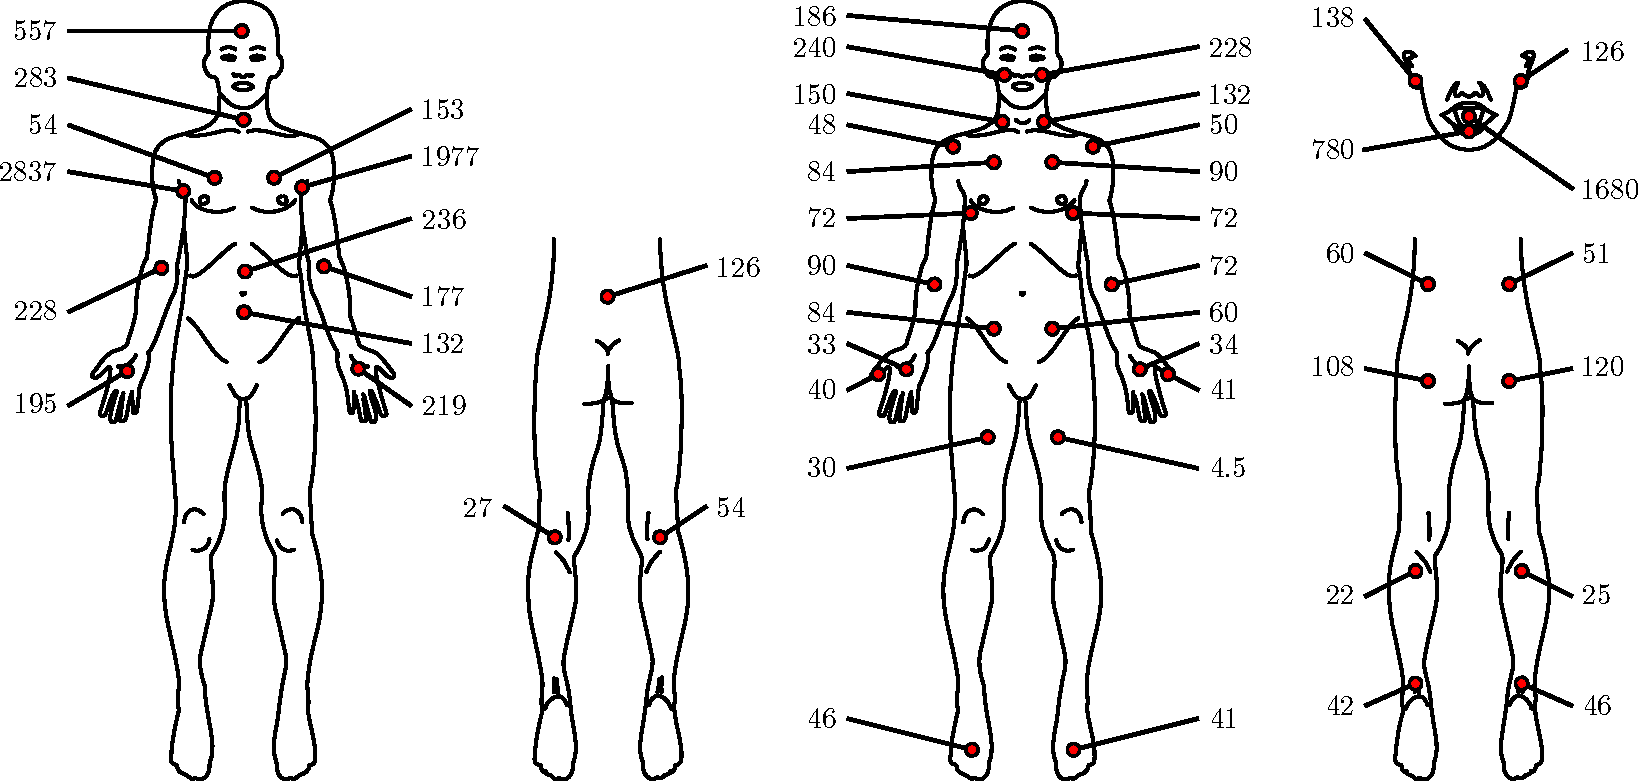
\includegraphics[width=\linewidth]{1_main_matter/tcco2_figures/positioning.pdf}
	\caption[\gls{co2} diffusion rates through human skin at various sites retrieved from the literature.]{\gls{co2} diffusion rates through human skin at various sites, expressed in cm$^3$.m$^{-2}$.h$^{-1}$, adapted from \cite{adamczyk1966} (\textbf{Left}) and \cite{levshankov1983} (\textbf{Right}).}\label{fig:tcco2:positioning}
\end{figure}

The high variability in Adamczyk's data---probably caused by the inclusion of only one subject---is glaring, especially when studying left-body / right-body differences. Interesting are the extremely important values reported for the axilla. These values may be measurement artefacts, or they may be caused by a peculiar behaviour towards \gls{co2} diffusion of the apocrine glands, which are mainly located in the axilla---see Baker \etal{}\cite{baker2019}. Another possibility could be the local production of \gls{co2} by the axilla's bacterial flora---through either aerobic respiration or fermentation---adding to the transcutaneously-diffused \gls{co2}\cite{taylor2003}. However, we found no evidence in the literature for or against these hypotheses. Alternatively, those elevated values may be caused by the skin temperature, which is much higher at the axilla on resting subjects than at the extremities\cite{niu2001, sund2002}, since the skin was not heated in their study. By contrast, the results of Levshenkov \etal{} are more homogenous concerning left and right body measurements.

All in all, and apart from the extreme axilla values, the reported \gls{co2} diffusion rates exhibit no extreme variations and are of the same order of magnitude, regardless of the measurement site. In this aspect, \textbf{it thus seems from the limited information at our disposal that no measurement site is far better than any other} from the \gls{co2} diffusion rate perspective. Consequently, we chose our measurement sites mainly for their ease of access and acceptability, with a view to using these sites for a future wearable \gls{ptco2} sensor. In this respect, the dorsal side of the wrist and the upper arm were found to be particularly interesting, as evidenced by the rapidly expanding and widespread use of health-related wristbands and armbands in the recent years\cite{eidan2018, soon2020, cosoli2020}.

\subsubsection{Skin \texorpdfstring{\gls{co2}}{CO2} Conductivity}

\paragraph{Metric Choice}\label{sect:tcco2:k_metric_choice}\mbox{}\\

It must be emphasised here that in the simplified skin diffusion model introduced in Section~\ref{sect:tcco2:modelling_tc_sensing} and detailed in Figure~\ref{fig:tcco2:diffusion_model}, the membrane called \enquote{skin} does \emph{not} correspond to an actual physiological membrane. Consequently, its thickness $w$ and diffusivity towards \gls{co2} does \emph{not} correspond to any physical property that might have been measured on a specific part of the dermis or epidermis. Rather, this \enquote{skin} membrane corresponds to a physical modelling of gas transport between the subcutaneous tissues and the outer air. As such, the latter membrane models both the diffusion of \gls{co2} through the stratum corneum \emph{and} the circulation of blood and diffusion of \gls{co2} in the dermis and subcutaneous tissues.

Moreover, this model also integrates the difference in \gls{ptco2} between that measured by the reference Radiometer \gls{ptco2} monitor, and that measured at the sensor's location. Indeed, since the reference \gls{ptco2} monitor was set to 41{\degree}C, it is likely that the \gls{ptco2} that we injected in Equation \ref{eq:tcco2:k_def} is slightly \hl{under}-estimated---as per the dilution principle presented in Figure \ref{fig:tcco2:barycentre_principle}---at temperatures below 41{\degree}C. Consequently, reported $K$---or $Q$---values below 41{\degree}C are likely to be slightly over-estimated. The amplitude of this over-estimation should be in the same order of magnitude as the arterio-venous \gls{pco2} gradient in resting, healthy subjects---\ie{} about 5--15\% in the \gls{nh}--38{\degree}C skin temperature range\cite{kowalchuk1988, schneider2013}. \mfrin{}However, this state of fact was inevitable since, to the best of our knowledge, no clinical \gls{ptco2} monitor working at a temperature below 37{\degree}C exists at the time being, and manufacturers recommend using 41--42{\degree}C---an injunction that we followed. Future research aiming at extending our work may consider the design of a \gls{ptco2} sensor working at low temperature in order to be able to perform the appropriate corrections to the so-obtained $K$ values.

\paragraph{Impact on the Response Time of a Future \texorpdfstring{\gls{ptco2}}{tcpCO2} Sensor}\label{subsect:tcco2:future_rt}\mbox{}\\

Contrary to perfusion---which increases over elevenfold with skin heating---$K$ only doubles from \gls{nh} to 44{\degree}C, and its increase is even smaller between 35--38 and 44{\degree}C values. This latter fact is all the more interesting when having in mind the design of a future energy-efficient \gls{ptco2} sensor. Indeed, internal studies measuring skin temperature under a wearable device (Bora Band, \bscy{}, France) positioned at the upper arm on ten healthy subjects revealed that a mean skin temperature of 33.9{\degree}C (range: 31.9--35.8{\degree}C, SD: 1.7{\degree}C) could easily be achieved at the upper arm without additional heating, and that covering the arm with an additional layer of isolation---\ie{} shirt or jumper sleeves---makes it rise even higher to reach 35.1{\degree}C (range: 34.5--36.6{\degree}C, SD: 0.58{\degree}C).

% wrist: 
% covered Avg.: 35.14°C	 min/max,	SD: 34.52/36.64°C, 0.58

With such skin temperatures, there is no strong incentive---from a response time point of view---to heat the skin actively any further---\ie{} by means of an external electrical heating system. Indeed, the measured increase of 35\% in $K$ at the arm from 35 to 44{\degree}C---see Figure \ref{fig:tcco2:ks_boxplot}---would result in a decrease in response time of the same magnitude for a given \gls{ptco2} sensor, according to the response time model presented in Section~\ref{sect:tcco2:modelling_tc_sensing}. While having a slower sensor may seem like a burning issue for critical care applications, it is not the case for telemonitoring for which long-term trends are to be observed over several months\cite{jang2021}.

Additionally, it should be noted that since the $Q$ values measured in the present study---80--178~cm$^3$.m$^{-2}$.h$^{-1}$ on average---are in line with that used in Section~\ref{sect:tcco2:modelling_tc_sensing} for response time calculations---100~cm$^3$.m$^{-2}$.h$^{-1}$---the afore-proposed sensor thickness of 100~{\textmu}m for a response time below 10~min remains credible. Of note, and to the best of our knowledge, there is a lack of clinical guidelines specifying the required response time for \gls{ptco2} monitors. Nevertheless, there exists a considerable amount of literature focusing on transcutaneous monitor testing in clinical environments, from which it can be inferred that a typical \invitro{} 90\% response time of about 1~min is achievable with current \gls{ptco2} monitors\cite{bendjelid2005, eberhard2007}. \textit{In vivo} performance reports, on their part, mention an approximatively 10~min initial equilibration time before a first \gls{ptco2} reading can be obtained\cite{carter2000, domingo2010, restrepo2012}. Regarding the response time of \gls{ptco2} monitors following a sudden change in \gls{paco2}, a lag has been reported in the literature between end-tidal \gls{pco2}---\ie{} \gls{petco2}---\gls{paco2}, and \gls{ptco2}, inducing a higher \invivo{} response time than in the ideal \invitro{} case. Reported values for this latter lag fall within the 1--5~min range\cite{kesten1991, carter2000, cuvelier2005, rafl2018}. An overall response time requirement of approximatively 5~min can thus \textit{de facto} be assumed for a \gls{ptco2} monitor to meet field expectations. Still, this latter assumption mainly holds for the intensive care of critically ill patients\cite{mari2019} and no information exists concerning long-term \gls{ptco2} (tele-)monitoring for the obvious reason that the corresponding monitors do not exist yet.

\subsubsection{Exhalation Rate}\label{subsect:tcco2:dis_skin_conduct}

\paragraph{An Imperfect Metric}\label{sect:tcco2:q_metric_choice}\mbox{}\\

Considering Equation~\ref{eq:tcco2:equa_diff_comp}, it readily appears that the exhalation rate $Q$ is not constant, and logically depends on the initial \gls{pseco2}, and on the passing of time. This issue has however been largely ignored by the literature on the topic---see Table \ref{table:tcco2:diff_rate_lit}---and $Q$ has been considered by most authors as if it had a single constant value. The latter, which has been reported as \emph{the} \gls{co2} diffusion rate through the skin, is actually the \emph{initial one in free air}---\ie{} Q(t=0) with \gls{pseco2}$(t=0)\approx 0$---and corresponds to the slopes of the tangents to the \gls{pseco2} curves at $t=0$ in Figure~\ref{fig:tcco2:rate_principle}, Left.

\begin{figure}
	\centering
	\includegraphics{1_main_matter/tcco2_figures/tikz/out/rate_ramp_up.pdf}
	\caption[\gls{pseco2} ramp up in single- or multiple-temperatures measurement scenarios.]{\textbf{Left:} schematic evolution of the \gls{pco2} inside the sensor's chamber when the skin is heated or not. \textbf{Right:} same as Left, but with a non-heated sensor placed onto the skin for a duration $t_\text{H}$ before being heated. Note the difference between the two sensing schemes: the one on the left requires two successive measurements---one heated, the other one non-heated---while the one on the right consists in a single measurement during which the skin is successively non-heated and then heated. The dashed line on the right represents what would have happened without heating during the whole acquisition, which is equivalent to the solid blue line on the left.}\label{fig:tcco2:rate_principle}
\end{figure}

Unfortunately, if measuring $Q$ as illustrated in the latter figure is theoretically feasible at different temperatures, it would also require to remove the sensor at each temperature change, in order to renew the gas inside the inner chamber of the sensor with fresh air. This would in turn require to peel off the sensor from the subject's skin at each temperature change, which would distort the $Q$ measurement, as the skin---and more specifically the \textit{stratum corneum}, its outermost layer---would become thinner and thinner after each sensor replacement. Actually, stripping the skin with multiple tape applications and removals is a well-known technique to drastically increase $Q$\cite{scheuplein1976, eletr1978, greenspan1981}.

Thus, the sensor was left in place in this study, while the temperature was successively changed from \gls{nh} up to 35, 38, 41, and finally 44{\degree}C. This led to measured \gls{pseco2} values with a similar appearance to those represented in Figure \ref{fig:tcco2:rate_principle}, Right. In that case, using $Q$ as a metric would be unpractical, since the \gls{pseco2} value at $t_\text{H}$ is not null, and $Q$ values would no longer represent \emph{initial} \gls{co2} diffusion rates as measured in free air. In practice, the $Q$ values obtained at different temperatures would then not be comparable with each other, each one being measured with a slightly different \gls{pseco2} initial value.

\def\arraystretch{1.25}
\begin{table}
	\centering
	\begin{tabular}{c|c|c|l}
		Exhalation Rate $Q$ & Temp. & Num. of & Ref. \\
		{[}cm$^{3}$.m$^{-2}$.h$^{-1}$] & [{\degree}C] & Subjects & \\ \hhline{=|=|=|=}
		25--120 		& 22--36 (air)	& 2 & Shaw (1929)\cite{shaw1929} \\ \hline
		10--160 		& 25--37 (air)	 & 1 & Shaw (1930)\cite{shaw1930} \\ \hline
		\textbf{58--169}			& \textbf{26--31 (air)}	& \textbf{38} & \textbf{Ernstene (1932)\cite[Table~1]{ernstene1932a}} \\ \hline
		12--143			& 23--37 (air)		& 1	& Whitehouse (1932)\cite{whitehouse1932} \\ \hline
		\textbf{32--69} & \textbf{25--28 (air)} & \textbf{13} & \textbf{Schulze (1943)\cite[Table~12]{schulze1943}} \\ \hline
		180--2500$^{(\dagger)}$	& -- 	 & 1 & Adamczyk (1966)\cite{adamczyk1966} \\ \hline
		25--87			& -- 				 & 5 & Thiele (1972)\cite{thiele1972} \\ \hline
		11--28 & 25--35 (air) & 3 & Frame (1972)\cite{frame1972} \\ \hline 
		\textbf{50} & \textbf{--} & \textbf{27} & \textbf{Levshankov (1983)\cite{levshankov1983}} \\ \hline
		\textbf{140--221} & \textbf{36 (skin)} & \textbf{14} & \textbf{E{\"o}ry (1984)\cite{eory1984}} \\ \hhline{=|=|=|=}
		25--192 & 27--32 (skin) & 40 & This work, \gls{nh} arm \\ \hline
		24--141 & 25--33 (skin) & 40 & This work, \gls{nh} wrist \\ \hline
		25--288 & 27--44 (skin) & 40 & This work, all temp. arm \\ \hline
		24--300 & 25--44 (skin) & 40 & This work, all temp. wrist
	\end{tabular}	
	\caption[\gls{co2} exhalation rates through the skin in the literature.]{\gls{co2} exhalation rates through the skin in the literature compared with the present studies. Past studies with more than ten participants are indicated \textbf{in bold} and were used for sample size determination. ($\dagger$): Axilla measured value, possibly erroneous.}\label{table:tcco2:diff_rate_lit}
\end{table}

\subsubsection{\texorpdfstring{Laser Doppler Flowmetry}{LDF}}

\paragraph{Choosing \texorpdfstring{nSkBF$_{90}$}{nSkBF90} as a Metric}\mbox{}\\

Both inter-subject and inter-site \gls{ldf} variabilities have often been reported in the literature\cite{johnson1984, cracowski2006, roustit2012, minson2010, hodges2016, cracowski2016}, and appear to be inherent to this modality of skin blood flow measurement, as well as to human physiology in general. Nonetheless, certain guidelines may be followed to obtain the most reproducible results\cite{cracowski2006}. In particular, when it comes to derive a single explicit \gls{ldf} metric from a given measurement period---such as a skin-site / sensor-temperature pair, for instance---several techniques have been developed to obtain meaningful results from raw \gls{ldf} data.

At first, some authors---\eg{} Hodges \etal{}\cite{hodges2016}---prefer to express the skin blood flow as \gls{cvc}, which is given by the \gls{ldf} in \gls{punit} or V, divided by the \gls{map}. The \gls{cvc} is said to be more \enquote{physiological}\cite{cracowski2006}, since an increase in skin blood flow could be caused by an increase in \gls{map} but also by an increase in vascular compliance, for instance. By dividing the \gls{ldf}-acquired blood flow by the \gls{map}, the obtained \gls{cvc} value is thus in theory more representative of the arteriovenous compliance, a theory supported by several works in haemodynamics\cite{johnsonpc1986, lautt1989, herring2018levick}. At the same time, skin blood flow alone---often abbreviated as SkBF, and either expressed in \gls{punit} or Volts---has been used for several decades\cite{johnson1984, frantz2012} and remains a good alternative to \gls{cvc} when \gls{map} is not available.

Then, once the type of measurement---SkBF or \gls{cvc}---is chosen, the question that comes next is that of the extraction of a single perfusion metric from a long-lasting acquisition. Indeed, due to the peculiar dynamics of thermal hyperaemia---see Figure~\ref{fig:tcco2:doppler_principle}, above---a simple time-averaging over the whole acquisition duration would make little sense.

To circumvent this issue, several research teams used temporal averaging on manually-set periods of interest in the raw \gls{ldf} data. The averaging duration that they used depended on the studied phenomenon, with durations of 1--3~min for transient phenomena---\ie{} initial bump and after-bump nadir---up to 5--10~min for long-lasting ones---\ie{} baseline or maximum perfusion plateau\cite{minson2001, frantz2012}. Other authors, for their parts, chose to average the 2--3 last minutes of a 10--25~min measurement window at the maximal perfusion value, the obtention of which is detailed below\cite{kellogg2008, hodges2016}. However, Barcroft, Taylor, \etal{}\cite{barcroft1943, taylor1984} mentioned even longer durations for thermal hyperaemia to fully settle following a change in skin temperature---up to 40--60~min. Such a lengthy onset period would result in a total acquisition duration in the 3--5~h range for the five different temperatures involved in the present study. On the contrary, a total experiment duration---including informing the subjects and obtaining their consent---of about 2~h seemed to us to be an acceptable maximum for easily recruiting volunteers. This 2~h duration in turn entails that each temperature window of the present study only lasted 18~min, which may not be enough for the establishment of the nitric-oxide mediated hyperaemia detailed in Figure~\ref{fig:tcco2:doppler_principle}. Thankfully, this 18~min duration is by far long enough for the axon mediated response to take place, and the latter often yields perfusion levels comparable to that reached at the end of the nitric-oxide mediated phase\cite{kellogg2008, minson2010, frantz2012,}. Thus, by taking the 90-th percentile of SkBF---see Section \ref{subsect:tcco2:subcut_bf}---the obtained SkBF$_{90}$ values are likely to be representative of the SkBF plateau values which would have been observed by increasing the duration of each temperature window. The latter hypothesis is further confirmed by the similarity between our results and that of the literature, as discussed in the next section.

Finally, it is also common practice to normalise the measured skin blood flow---whether expressed as SkBF or \gls{cvc}---by its maximum value, often taken after a prolonged ($\geq$15~min) period at an elevated ($\geq$44{\degree}C) temperature\cite{taylor1984, vionnet2014, hodges2016} or by direct injection of sodium nitroprusside\cite{kellogg2008}. Although it has been occasionally proposed to normalise the measured values by the baseline blood flow value instead of the maximum one\cite{magerl1996, mayrovitz2001}, this is considered bad practice because intra-subject baseline variations can be far from negligible, even in a temperature controlled room\cite{bircher1994, cracowski2006}.

In this study, \gls{cvc} was not considered due to the invasiveness of a continuous \gls{map} measurement, and SkBF was thus chosen as raw perfusion metric. Then, we proposed to take the 90-th percentile of a given temperature window instead of time averaging. Finally, normalisation by the maximum perfusion value---\ie{} the one reached at the end of the 44{\degree}C window---was performed, as per literature guidelines.

\paragraph{Comparison With the Literature}\mbox{}\\

The \gls{ldf} measurements that were gathered in the present study are consistent with existing literature on the topic. In particular, the sigmoid behaviour observed in Figure \ref{fig:tcco2:nskbf_boxplot}---revealing a strong onset of hyperaemia in the 35--41{\degree}C range---is on par with the observations of Magerl, Stephens, Hodges \etal{}\cite{magerl1996, stephens2001, hodges2016}.

\paragraph{Impact on the Accuracy of a Future \texorpdfstring{\gls{ptco2}}{tcpCO2} Sensor}\label{subsect:tcco2:frontiers:acc_impact}\mbox{}\\

The fact that the perfusion is doubled at 35{\degree}C and quadrupled at 38{\degree}C compared to baseline---see Figure \ref{fig:tcco2:nskbf_boxplot}---is especially encouraging for the development of a future energy-efficient \gls{ptco2} sensor, since these temperatures can be easily achieved without---or with minimal---heating, as already discussed in Section \ref{subsect:tcco2:future_rt} (reaching over 35{\degree}C at the upper arm under jumper sleeves). Indeed, since arterialised capillary blood---either obtained by local heating or by applying a vasoactive cream---is gaseously close to arterial blood\cite{zavorsky2007}, it is to be expected that partially arterialised capillary blood obtained by a mild heating---\ie{} below 44{\degree}C---lies somewhere between venous and arterial blood, from a gaseous content point of view. More specifically, Rooth \etal{}\cite{rooth1987} hypothesised that the subcutaneous capillary \gls{pco2}---\ie{} \gls{ptco2}---would be a barycentre between venous and arterial \gls{pco2}, as illustrated in Figure \ref{fig:tcco2:barycentre_principle}.

\begin{figure}
	\centering
	\includegraphics{1_main_matter/tcco2_figures/tikz/out/barycentre_principle}
	\caption[Capillary \gls{pco2} as a function of relative blood flow considering two venous \gls{pco2} levels: at rest, and while exercising.]{Capillary \gls{pco2} as a function of relative blood flow considering two venous \gls{pco2} levels: at rest, and while exercising. Relative blood flow values measured in the present study were also added in red with their respective temperature labels. A normal \gls{paco2} of 40~mmHg\cite{schneider2013} was taken for arterial blood, while venous blood levels were set to 46 and 60~mmHg at rest and while exercising, respectively. Of note, while 46~mmHg at rest is generally accepted in the literature\cite{byrne2014}, the 60~mmHg exercising value was mainly chosen for legibility reasons. Indeed, exercising values may exceed 100~mmHg during heavy exercise, or in case of septic shock\cite{kowalchuk1988, diaztagle2017}. Modified from Rooth \etal{}\cite{rooth1987}.}\label{fig:tcco2:barycentre_principle}
\end{figure} % additional citations ekstrom, malinoski, tregger, walkey dans skinCO2, biblio physio, blood

This figure emphasises the fact that---especially for a resting subject---even a mild heating of the skin in the 35--38{\degree}C range could be enough to yield a \gls{ptco2} only a few mmHg away from the \gls{paco2}. Such a small error may be acceptable depending on the clinical application targeted. For example, the \gls{fda} requires \gls{ptco2} monitors to be accurate within 5~mmHg, with an allowed drift of up to 10\% of the initial reading over a one-hour period\cite{fda_transcut}.

\subsubsection{Sample size}\label{subsect:tcco2:sample_size}

The main objective of the present study was to estimate the mean $K$ value as a function of temperature. The latter mean can be estimated at each temperature $T$ by
\begin{equation}
	\widehat{K}_{T} = \frac{1}{N} \cdot \sum_{i=1}^{N} K_{S,i}
\end{equation}
wherein the $i$ index stands for the $i$-th subject of the study, and $N$ stands for its sample size. Contrary to hypothesis testing, for which a sample size may be derived straightforwardly from targeted alpha or beta risks and some prior knowledge of the data\cite[Chap.~19]{ambrosius2007topics}\cite{chow2017sample}, sample size determination in the case of an exploratory---or pilot---study is more challenging, with its share of arbitrary decisions\cite{ko2021}. Indeed, while a 95\% confidence interval can be computed for $K_T$ as
\begin{equation}\label{eq:tcco2:ci_def}
	C.I._{K_T}^{95\%} = [\widehat{K}_{T} - \varepsilon, \widehat{K}_{T} + \varepsilon], \quad \text{and} \quad \varepsilon = - t_{N-1}\left(\frac{0.05}{2}\right) \cdot \frac{s}{\sqrt{N}}
\end{equation}
wherein $t_{N-1}$ is the percentile score of a Student distribution with $N-1$ degrees of freedom, and $s$ is the \gls{sd} of the sample---\ie{} the \emph{estimated} standard deviation of the population---the value of the latter \gls{sd} is vastly unknown. In order to estimate an adequate sample size for the study at hand---based on an \emph{acceptable} margin of error on $\widehat{K}_T$---a prior estimation of $s$ is thus needed, and is the object of the upcoming section. Importantly, since $Q$---that is $Q(t=0)$ using the above-presented notation---was studied by earlier authors instead of $K$, the following reasoning will be made using the former. This can be done safely since the two values are linked by a proportionality constant---see Equation \ref{eq:tcco2:k_def}. Of note, Equation \ref{eq:tcco2:ci_def} holds only if $K_T$ follows a normal distribution, which has neither been confirmed nor denied in the literature, to the best of our knowledge, but which has been verified in the current study---see Section \ref{subsect:tcco2:ss_result}.

\paragraph{Literature Review}\mbox{}\\

Among the literature studies on the topic of skin \gls{co2} exhalation rate measurements on human subjects detailed in Table \ref{table:tcco2:diff_rate_lit}, only four of them have been performed on more than ten subjects. Those four studies are highlighted \textbf{in bold} in the aforementioned table. Unfortunately, the latter studies are sometimes unclear about $Q$ measuring conditions---measurement site and skin temperature, in particular. We did our best not to distort or misinterpret the works of their authors, but what follows is essentially our best \emph{interpretation} of their writings. These four studies reported---or made it possible to derive from raw data---a $\widehat{Q}$ and $s$ value for each measurement site investigated. These data can be used to compute 95\% confidence intervals on $Q$ estimation---as shown in Equation \ref{eq:tcco2:ci_def}---or on $s$, yielding the following expression\cite[Chap.~4]{ambrosius2007topics}:
\begin{equation}\label{eq:tcco2:sigma_ci}
	C.I._{\sigma}^{95\%} = \left[ \frac{s^2 \cdot (N-1)}{\chi^2_{N-1}\left(\frac{0.05}{2}\right)} \ ; \ \frac{s^2 \cdot (N-1)}{\chi^2_{N-1}\left(1 - \frac{0.05}{2}\right)} \right]
\end{equation}
wherein $\chi^2_{N-1}$ is the percentile score of a $\chi^2$ distribution with $N-1$ degrees of freedom. The resulting confidence intervals are reported in Table \ref{table:tcco2:indic_estimation} and tend to indicate a relative uncertainty on $Q$ estimation in the order of 5--30\% for relatively small sample sizes---\ie{} 13--38 subjects.

\def\arraystretch{1.25}
\begin{table}
	\centering
	\begin{tabular}{c|c|c|c|c|c|c}
		& \specialcell{Lower\\bound} & Reported & \specialcell{Upper\\bound} & \specialcell{Relative \\uncertainty} & \specialcell{Measurement\\site} & Ref. \\ \hline
		\multirow{6}{*}{$\sigma$} & 18.7 & 22.9 & 29.6 & 48\% & Whole arm & Ernstene (1932)\cite{ernstene1932a} \\
		& 8.5 & 11.9 & 19.6 & 93\% & Abdomen & Schulze (1943)\cite{schulze1943} \\
		& 2.65 & 3.36 & 4.60 & \multirow{2}{*}{58\%} & Left forearm & Levshankov (1983)\cite{levshankov1983} \\
		& 2.41 & 3.06 & 4.19 & & Right forearm & Levshankov (1983)\cite{levshankov1983} \\
		& 15 & 21 & 34 & \multirow{2}{*}{89\%} & Acupuncture site & E{\"o}ry (1984)\cite{eory1984}\\
		& 13 & 18 & 28 & & \enquote{adj. skin area} & E{\"o}ry (1984)\cite{eory1984} \\ \hline
		\multirow{6}{*}{$Q$} & 113 & 120 & 128 & 13\% & Whole arm & Ernstene (1932)\cite{ernstene1932a} \\
		& 41 & 48 & 55 & 30\% & Abdomen & Schulze (1943)\cite{schulze1943} \\
		& 48.0 & 49.3 & 50.7 & 5.39\% & Left forearm & Levshankov (1983)\cite{levshankov1983} \\
		& 48.4 & 49.6 & 50.8 & 4.88\% & Right forearm & Levshankov (1983)\cite{levshankov1983} \\
		& 209 & 221 & 233 & 11\% & Acupuncture site & E{\"o}ry (1984)\cite{eory1984} \\
		& 130 & 140 & 150 & 14\% & \enquote{adj. skin area} & E{\"o}ry (1984)\cite{eory1984}
	\end{tabular}	
	\caption[Confidence intervals at the 95\% level for $\sigma$ and $Q$.]{Confidence intervals at the 95\% level for $\sigma$ and $Q$, computed from $s$ and $\widehat{Q}$ values reported in the literature. Aside from the relative uncertainties---defined as $2\cdot\varepsilon/X$ wherein $X$ is $\sigma$ or $Q$---all values are given in cm$^{3}$.m$^{-2}$.h$^{-1}$.}\label{table:tcco2:indic_estimation}
\end{table}

\paragraph{Chosen Sample Size}\mbox{}\\

The reported $s$ value, as well as the upper and lower bounds of its 95\% confidence interval, were then used to compute the relative uncertainty on $Q$ as a function of the number of subjects, using Equation~\ref{eq:tcco2:ci_def}. While this relative uncertainty decreases when the sample size increases, its reducing rate---as well as the associated uncertainty values---varies wildly depending on the considered data source. Indeed, while a sample size of 20--30 subjects should lead to a relative uncertainty on $Q$ in the 5--10\% range using Levshankov \etal{} data, much larger sample sizes---\ie{} 100--150 subjects---would be needed to reach the same level of accuracy using Schulze, or Ernstene \etal{} measurements. In the end, since the works of the latter two authors were much older---1932 and 1943, respectively---than that of Eöry, Levshankov \etal{}---1983 and 1984, respectively---it was decided to put them aside. The sample size determination for the present study was thus grounded only on the works of Eöry, Levshankov \etal{}, and a sample size of 40 subjects was deemed acceptable, since it should have resulted into a relative uncertainty on $Q$ estimation below 10\%.

\paragraph{Results}\label{subsect:tcco2:ss_result}\mbox{}\\

Unfortunately, this initial estimation of a 40 subjects cohort proved to be rather optimistic in practice. Indeed, the relative uncertainty on measured $Q$ values can be computed using Equation \ref{eq:tcco2:ci_def}, and falls in the 15--32\% range, depending on the skin temperature and measurement site. In this aspect, our results are close to those presented by Ernstene, Schulze, Eöry \etal{}\cite{ernstene1932a, schulze1943, eory1984} who report relative uncertainties in the 11--30\% range. Yet, the latter authors used less than 40 subjects, and our uncertainty ranges were thus expected to be narrower than theirs. Moreover, the present study also exhibits a higher variability than that of Levshankov \etal{}\cite{levshankov1983}---whose results indicate a relative uncertainty of only about 5\%, see Table \ref{table:tcco2:indic_estimation}.

The origin of these discrepancies between literature-driven expectations and the above-presen\-ted results is not fully understood at the moment. One possible explanation could be differing measurement sites between the above-mentioned studies and the ones that we chose. Indeed, the data reported by Eöry and Schulze (Table 16 \textit{op. cit.}) tend to indicate some degree of variability in the relative uncertainty expected at different sites---in particular when comparing the abdomen and hand in Schulze's data (30 \textit{vs.} 45\%), or the two sites used by Eöry (10 \textit{vs.} 14\%). Thus, it seems plausible that $Q$ variability at the upper arm and wrist is larger than that reported in earlier studies for differing sites.

Ultimately, we cannot but recommend using larger sample sizes in future studies of a similar nature, considering the significant variability that we observed. As a side note related to sample size determination, the normality of the $Q$ distribution was ascertained using a series of Bonferroni-corrected Shapiro-Wilk tests which were non-significant, further justifying the approach presented in Section~\ref{subsect:tcco2:sample_size}. To the best of our knowledge, this is the first report of normality for transcutaneous \gls{co2} exhalation rates.

\subsection{Conclusion}\label{sect:conclusion}

As stated in Section~\ref{sect:tcco2:frontiers_intro}, the aim of this study was twofold: measuring the influence of skin temperature on the transcutaneous diffusion of \gls{co2}, and on the skin blood flow. To this end, a custom sensor was designed and used on 40 healthy human subjects at two measurements sites: the upper arm, and the wrist.

Our results indicate comparable behaviours at both sites, with an increasing relationship between temperature on the one hand, and \gls{co2} exhalation rate, \gls{co2} conductivity and perfusion on the other hand. These results are encouraging for the development of a future energy-efficient \gls{ptco2} sensor for the following reasons:

\begin{itemize}
	\item[--] Skin conductivity towards \gls{co2} increases only moderately with an increase in skin temperature, at most doubling from \gls{nh} to 44{\degree}C. Thus, if the response time of the sensor-to-be is not critical---\ie{} if a 35\% slower response is acceptable compared to the one reachable at maximum skin heating---the latter may not require additional heating. This is especially encouraging in the perspective of building a wearable, battery-operated device.
	\item[--] Perfusion, for its part, increases strongly with an increase in skin temperature, already doubling from \gls{nh} to 35{\degree}C, and quadrupling from \gls{nh} to 38{\degree}C. This phenomenon is especially interesting since---according to Rooth \etal{}\cite{rooth1987}---this should bring \gls{ptco2} close to \gls{paco2} even for skin temperatures as low as 35--38{\degree}C, which are reachable at the arm without additional heating provided that the latter is covered by warm clothings. \mfrin{}However, this latter hypothesis---\ie{} the existence of a clinically-satisfying \gls{ptco2} / \gls{paco2} correlation in the 35--38{\degree}C skin temperature range---is yet to be demonstrated experimentally \invivo{}, which will be the subject of future research.
\end{itemize}

Additionally, our results highlight the significant variability of transcutaneous \gls{co2} exhalation rate and conductivity measurements in human subjects. Hence, we strongly advise future research on the topic to consider large sample sizes---\ie{} more than 40 subjects---in order to ensure accurate estimates of the latter metrics. The present study also focused only on two measurement sites---the upper arm and the wrist---and further investigations at other sites would be welcome. In particular, the remarkably high axilla values reported by some authors is intriguing, and could benefit from a special attention. Of note, the study's data---demographics, $K$, $Q$, and nSkBF$_{90}$ values---were provided as Supplementary Materials in the original paper\cite{dervieux2023rate}, and are also available \hl{in this thesis' repository}.

\section{Cutaneous Measurement Conditions}\label{sect:tcco2:skin_conditions}

While the previous section focused solely on the transcutaneous \gls{co2} diffusion, this section addresses other conditions affecting cutaneous measurements. In particular, the following factors are considered:
\begin{multicols}{2}
	\begin{itemize}
		\item[--] temperature, in Section \ref{sect:tcco2:skin_mes:temp},
		\item[--] humidity, in Section \ref{sect:tcco2:skin_mes:rh},
		\item[--] \gls{po2}, in Section \ref{sect:tcco2:skin_mes:po2}, and
		\item[--] acidic compounds, in Section \ref{sect:tcco2:skin_mes:acid}.
	\end{itemize}
\end{multicols}

\subsection{Skin Temperature}\label{sect:tcco2:skin_mes:temp}

Skin temperature has been measured by several authors---including myself---on human subjects. Early studies conducted on one subject by Benedict \etal{}\cite{benedict1919} in 1919, and on 15 subjects by Barcroft \etal{}\cite{barcroft1943} in 1943 reported forearm temperatures averaging at 33.3{\degree}C and 33.0{\degree}C, respectively. A more recent work performed by Zhu \etal{}\cite{zhu1999} in 1999 on 223 subjects (138 male, 85 female) presents mean temperatures of 32.3{\degree}C at the forearm, and 31.4{\degree}C and 31.1{\degree}C at the right and left wrists, respectively. Several studies made at the university of Murcia in Spain in  2008\cite{sarabia2008}, 2012\cite{blazquez2012} and 2013\cite{martinez2013} on 99 subject, 28 subjects and 103 subjects by the same research team report mean wrist temperatures of 34.0{\degree}C, 33.7{\degree}C and 33.5{\degree}C, respectively. These latter studies, however, used a wristband to perform their measurements. Since this wristband prevents the heat produced by the wrist from being dissipated in the ambient air, temperatures in these studies were expected to be higher than in the afore-mentioned works.

Concerning studies that I performed internally on Biosency's employees who gave their informed consent, a first work on 18 resting subjects (12 male, 6 female) revealed bare skin temperatures at the wrist of 30.7$\substack{+2.2 \\ -2.5}${\degree}C at a room temperature of $22.5\substack{+0.6 \\ -0.9}${\degree}C. Measurements in the same conditions but under a wristband yielded temperatures of 31.9$\substack{+3.9 \\ -4.0}${\degree}C (mean computed over more than 30~min, after an 8~min ramp-up time). This increase of about 1{\degree}C is attributed to the supplementary isolation provided by the worn wristband. A second study was performed on 10 subjects (5 male, 5 female) at the upper arm under a shirt or jumper sleeve, and yielded a mean temperature of 35.1$\substack{+1.5 \\ -0.6}${\degree}C.

To sum up, in the absence of external heating and when uncovered, mean skin temperature may lie in the 31--33{\degree}C range at the wrist. When the skin is covered by a wristband, it heats up slightly to reach temperatures in the 32--34{\degree}C range. When the latter wristband is further covered by an additional clothing layer and moved to the upper arm, 35{\degree}C or above can reasonably be expected without active heating.

\subsection{Skin Humidity}\label{sect:tcco2:skin_mes:rh}

Human skin has a critical double barrier function: \emph{(i)} from the outside to the inside in order to prevent the introduction of foreign bodies, potentially harmful micro-organisms, and contaminants into the organism, and \emph{(ii)} from the inside to the outside, mainly to prevent excessive water losses, and the dehydration of the body in a dry environment\cite{ehrhardt2008}. Still, the skin remains significantly permeable to a variety of substances, including for instance gases, water vapour, drugs, and solvents\cite{scheuplein1976, schaefer1982}. In particular, water diffuses from the deeper layers of the skin towards its dryer outer layers, forming the so-called \gls{tewl}.

\subsubsection{Transepidermal Water Loss}\label{subsect:tcco2:tewl}

\gls{tewl} is defined as the amount of water leaving the skin per unit of time and surface, and is often expressed in g.m$^{-2}$.h$^{-1}$. Although it can be used as a metric to assess the proper barrier function of the skin\cite{montero2021}, there is no such think as a \enquote{normal} \gls{tewl} level, for which values have been reported in the 2.3--44.0~g.m$^{-2}$.h$^{-1}$ range, with wide variations across measurement sites\cite{kottner2013, akdeniz2018}. Additionally, several authors have noted that, strictly speaking, \gls{tewl} should be expressed without taking into account the water added by sweating\cite{rogiers2001, fluhr2004bioengineering}. Although this additional constraint has been ignored by a number of authors, some used a topical treatment---\eg{} poldine methylsulfate---to prevent sweating during \gls{tewl} measurements\cite{grice1972}. Preventing sweating may however not be that much of a concern, since heat-triggered sweating rates are usually orders of magnitude higher than reported \gls{tewl} values\cite{cheuvront2009}. As such, the pollution of \gls{tewl} measurements by the unwanted onset of sweating---if it occurred---could be easily detected.

\subsubsection{Variables Affecting the \texorpdfstring{\gls{tewl}}{TEWL}}

\gls{tewl} is affected by a number of variables, such as the measurement site, skin and probe temperatures, occlusion duration, presence of skin diseases, or subject's stress level, among others\cite[pp.~63--76]{fluhr2004bioengineering}\cite{aly1978, rogiers2001, li2015, schmuth2020}. A brief overview of these variables is given below:

\begin{itemize}
	\item[--] \textbf{Measurement site:} huge discrepancies exist between different body parts, with \gls{tewl} reported for the palm, forehead, and forearm about 38, 18 and 6~g.m$^{-2}$.h$^{-1}$\cite{rogiers1995}, for instance. More detailed comparisons of many more skin sites are available in the works of Fluhr, Akdeniz, Kottner \etal{}\cite{fluhr2004bioengineering, kottner2013, akdeniz2018}.
	\item[--] \textbf{Temperature:} the skin and probe temperatures also play an important role in the measurement of \gls{tewl}: the higher those temperatures, the higher the measured \gls{tewl}\cite{mathias1981, rogiers1995, cravello2008}.
	\item[--] \textbf{Humidity:} the ambient \gls{rh}, on its part, may play a role in \gls{tewl}, although conflicting studies exist in the literature: in the work of Grice \etal{}\cite{grice1972} the measured \gls{tewl} seems maximal at 25--50\% \gls{rh} but decreases for extremely low or high \gls{rh} values, whereas Sunwoo \etal{}\cite{sunwoo2006} report increasing \gls{tewl} values with a decreasing \gls{rh}.
	\item[--] \textbf{Occlusion:} occluding the skin greatly increases the \gls{tewl}, with early work by Aly \etal{}\cite{aly1978} reporting a three-fold increase in \gls{tewl} value after five days of occlusion under a \gls{pvdf} film. Other authors have also shown similar tendencies, as reported by Golda \etal{}\cite{golda2005} in an overview on the topic.
	\item[--] \textbf{Skin diseases:} as mentioned above, \gls{tewl} is a good indicator of the proper barrier function of the skin and, as such, may be used as a diagnostic tool for the screening of psoriasis or dermatitis\cite{laudaska2003, montero2021}. These diseases provoke a degradation of the skin and a decline in its barrier function, resulting in a significant increase in \gls{tewl}.
	\item[--] \textbf{Stress:} psychological stress \emph{may} induce modifications of the \gls{tewl}---conflicting sources---with a possible increase in \gls{tewl} values in case of skin disruption after an injury---\ie{} tape stripping---in the presence of psychological stress\cite{altemus2001, muizzuddin2003}. % Fukuda2014, c'est vraiment des connards...
\end{itemize}

All in all, these numerous sources of variations may explain the wide range of \gls{tewl} values reported in Section~\ref{subsect:tcco2:tewl}. In the context of this doctoral work, \gls{tewl} should be as high as possible to provide a quick hydration of the \gls{co2}-sensing patch introduced in the next chapter. Thus, the consequences of occlusion, skin diseases, or stress, may all be beneficial in effects. Temperature should not be an issue either, since skin temperature can easily be brought above 32{\degree}C without active heating---see Section~\ref{sect:tcco2:skin_mes:temp}---and because there is no further increase in \gls{tewl} with cutaneous temperatures above $\approx$30{\degree}C\cite{rogiers1995}. The measurement site, on its part, must be well-accepted by future patients, as mentioned in Section~\ref{sect:tcco2:frontiers:sensor_pos}, and in this respect the upper arm and wrist seem particularly suitable. However---and this is especially true for the upper arm---these two sites have relatively low \gls{tewl} values, compared to other body sites\cite{kottner2013, akdeniz2018}. Thus, the results presented below for \gls{rh} measurements at the upper arm, on healthy skin, and without heating or clothing, are expected to be a worst-case scenario.

\subsubsection{Experimental Validation}

\paragraph{Humidity Sensing Patch}\label{subsect:tcco2:skin_mes:rh:patch_description}\mbox{}\\

In order to evaluate reachable humidity levels under a gas-tight impermeable layer, a custom transcutaneous humidity testing patch was designed, inspired by the early work of Masaki \etal{}\cite{masaki1986}. The latter patch is presented in Figure \ref{fig:tcco2:humid_principle} and entraps four colorimetric sensing dots---which change colour at 20, 40, 60 and 80\% \gls{rh}---under a gas-tight polypropylene layer.

\begin{figure}
	\centering
	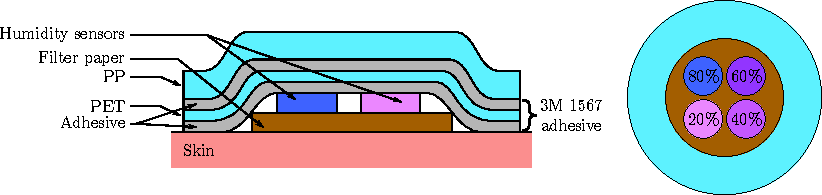
\includegraphics{1_main_matter/tcco2_figures/humid_patch_schem.pdf}
	\caption[Colorimetric humidity sensing patch schematic.]{Colorimetric humidity sensing patch. \textbf{Left:} cross-sectional view of the patch. From bottom to top: a filter paper disk is covered with colorimetric sensing dots (humidity sensors), a double sided layer of adhesive including an intermediary \gls{pet} backing, and a polypropylene (PP) covering film. \textbf{Right:} top view, showing the concentric design of the patch. The four colorimetric sensing dots are placed at the centre, above a filter paper disk, itself covered with a double-layer adhesive and a polypropylene film.}
	\label{fig:tcco2:humid_principle}
\end{figure}

All parts were hand-cut using a scalpel and a set of punches, and consist in:
\begin{itemize}
	\item[--] A top, gas-tight, 110~{\textmu}m thick and 31~mm in diameter, polypropylene layer (3365249, Office Depot, USA).
	\item[--] An intermediate, double-sided adhesive layer, also 31~mm in diameter, made out of two synthetic rubber-based pressure sensitive adhesive layers, coating a 20~{\textmu}m thick \gls{pet} film, for a total thickness of 130~{\textmu}m (1567, 3M, USA).
	\item[--] Four reversible, colorimetric, cobalt chloride-based, humidity sensing dots scavenged from humidity test strips (PGA05V50, Bartovation, USA), 200~{\textmu}m thick and 3~mm in diameter, which change colour from blue to pink depending on the \gls{rh} to which they are exposed. These four sensing dots switch to pink at 20, 40, 60 and 80\% \gls{rh}. Of note, due to the scavenging process---\ie{} peeling off the sensing patches using a scalper---the actual thickness of the dots was in the 110--190~{\textmu}m range (mean: 153~{\textmu}m).
	\item[--] A bottom layer of filter paper (100\% cellulose coffee filter {\textnumero}4$\times$80, Système U, France) to avoid direct skin contact with the sensing dots---as cobalt chloride is a potential allergen\cite{zug2009, thyssen2012}---100~{\textmu}m thick and 11~mm in diameter.
\end{itemize}

% 110μm thick PP
% from tock1983, PP for water: 0.5 g * mil / 24h / 100in²
% 0.5 / (110μm / 25.4 ) * (100/2.54)² / 100 / 24 = 0.075
%
% 20μm PET
% from tock1983, PET for water: 1.2 * mil / 24h / 100in²
% 1.2 / (20 / 25.4 ) * (100/2.54)**2 / 100 / 24 = 0.98

Note that given the low water vapour transmission rate of \gls{pet}---\ie{} 0.98~g.m$^{-2}$.h$^{-1}$ for a 20~{\textmu}m layer\cite{tock1983}---compared to reported \gls{tewl} values---2.3--44.0~g.m$^{-2}$.h$^{-1}$\cite{kottner2013, akdeniz2018}---it was considered in first approximation that water vapour stopped at the \gls{pet} layer and diffused no further. Thus, the thickness of the volume into which the water vapour diffuses from the skin is considered to be 308~{\textmu}m on average (100~{\textmu}m of filter paper, 55~{\textmu}m of adhesive, and 153~{\textmu}m of colorimetric sensing spot, on average). This approximation leads to pessimistic estimates of the amount of water diffusing from the skin to the outer air, and is therefore conservative. Indeed, considering the \gls{pet} layer as permeable would lead to a thicker equilibration volume, and thus to higher estimated water vapour diffusion rates.

\paragraph{Protocol}\mbox{}\\

Once built, the patches were stored in a dry environment, so that all sensing dots were blue at the beginning of the measurements. The sensing patches were then placed on the flat area located between the biceps, the triceps, and the lower part of the deltoid, on the dorsal side of the arm, as depicted in Figure \ref{fig:tcco2:patch_protoc}, Right. For illustration, two test strips in a dry and humid environment are also depicted in Figure \ref{fig:tcco2:patch_protoc}, Left, as well as a fully-assembled patch before application on a test subject, Center.

\begin{figure}
	\centering
	\includegraphics{1_main_matter/tcco2_figures/tikz/out/humid_patch.pdf}
	\caption[Colorimetric humidity sensing patch pictures.]{\textbf{Left:} two test strips, one equilibrated with ambient air at 59\% \gls{rh} (on the left) and the other one stored in a dry box (on the right). The sensing squares turn to pink (and are supposed to be read at lavender) at 20, 40, 60 and 80\% \gls{rh}---from top to bottom. Note how the left strip turned to pinkier tones---in particular, its 60\% square is lavender. \textbf{Center:} a fully assembled patch stored in dry air just before its application on a subject's skin. \textbf{Right:} the application site of the patch is on the flat area below the deltoid (circled in dashed red). Note how the applied patch has already partially changed colour to turn pink, lavender, and pale blue.}
	\label{fig:tcco2:patch_protoc}
\end{figure}

The studied population consisted of 10 human adults (5 male, 5 female) between 23 and 50 years of age (median age 33), all of whom signed an informed consent notice before the experimentation. The research was led indoor, with an ambient temperature in the {20.6--27.3}{\degree}C range and \gls{rh} levels in the {50.7--59.8}\% range, as measured using a calibrated Testo 174H data logger (Testo, Germany).

\paragraph{Results}\mbox{}\\

The outcomes of the experiment are summarised in Figure \ref{fig:tcco2:humid_results}. The 20\% and 40\% sensing dots all turned to pink or lavender within the first 10~min after application of the patches, and the 60\% sensing dots all turned to pink or lavender after only 20~min. However, the change in colour from blue to pink for the 80\% sensing dots took between 40 and 90~min, depending on the test subject, with a mean duration of 70~min. This wide range of humidity saturation times is not surprising though, considering the wide range of \gls{tewl} reported in the literature (see Section~\ref{subsect:tcco2:tewl}). It could also be partially explained by the discrepancies in the sensing dots thicknesses, as above-mentioned (see Section \ref{subsect:tcco2:skin_mes:rh:patch_description}).

\begin{figure}
	\centering
	\includegraphics[width=.95\linewidth]{1_main_matter/tcco2_figures/tikz/out/humid_results.pdf}
	\caption[Temporal evolution of the humidity sensing patches.]{Temporal evolution of the experiment. The coloured areas represent the number of blue, lavender, and pink sensing dots in a normalised stacked area chart. The red and black dashed line represents the number of subjects for whom all four sensing dots turned to pink, \ie{} those for whom the \gls{rh} under the patch is above 80\%.}
	\label{fig:tcco2:humid_results}
\end{figure}

Those results are particularly encouraging because the \gls{rh} easily reached over 80\% under the designed patch. Thus, the presence of water molecules for the hydration of \gls{co2} inside a fluorescent sensing patch such as that considered in the next chapter should not be a source of concern. As a result, \textbf{the design of fluorescence-based \gls{co2}-sensing thin films for \gls{ptco2} measurement can be performed considering \gls{rh} levels in the 80--100\% range}. The concerns expressed by several authors\cite{mills1997, malins1998, segawa2003, ge2003, fernandezsanchez2007, dansby2010} about the \emph{drying-out} of the film when used for ambient air \gls{co2} sensing can thus be safely ignored in the context of trans-cutaneous \gls{co2} sensing. These first results are also consistent with the findings of Matsumura \etal{}\cite{matsumura1995}, who noticed sweat drips forming under a low water permeability polymer film occluding human skin.

Then, the \emph{response time} of the humidity patches is also particularly interesting. Indeed, the mean time taken to reach a \gls{rh} level above 80\% was 70~min. Considering that the equilibration volume---\ie{} the equivalent air volume that is entrapped between the top layers of the sensing patch and the skin---to be filled by humid air is 308~{\textmu}m thick on average, a much shorter humidification time is expected for thinner patches. Indeed, a similar reasoning to that exposed in Section~\ref{sect:tcco2:modelling_tc_sensing} about \gls{co2} diffusion in an enclosed chamber can be followed for water vapour. In this case, the equilibration time is essentially a linear function of the thickness of the equilibration volume. Thus, the presented measurements imply an equilibration rate---\ie{} time taken to reach over 80\% \gls{rh} under a patch of given thickness---of 14~s.{\textmu}m$^{-1}$ on average\footnote{Value computed taking the average values of the equilibration time and dot thickness. Minimum value---shortest equilibration time with thickest dot---is 7~s.{\textmu}m$^{-1}$ and maximum value---longest equilibration time with thinnest dot---is 20~s.{\textmu}m$^{-1}$.}. This means that \textbf{the \gls{rh} under a \gls{co2} sensing patch could be over 80\% in a matter of minutes for sensing films 10--50~{\textmu}m thick}---\ie{} the thickness range envisioned for fluorescence-based \gls{co2}-sensing thin films in the next chapters.

\subsection{\texorpdfstring{\Gls{o2}}{O2} Diffusion}\label{sect:tcco2:skin_mes:po2}

\gls{o2} also diffuses through the skin, albeit typically in the opposite direction to \gls{co2}---\ie{} from the ambient air towards the tissues---since the \gls{po2} in tissues is necessarily lower than that in the ambient air. Normal transcutaneous \gls{o2} pressure varies strongly depending on skin temperature: for a skin heated at 37$\degree$C, values as low as 0.3--0.7~kPa have been reported\cite{ewald1981}, while at 45$\degree$C the \gls{tcpo2} mean value can reach 10.9~kPa\cite{wimberley1985a}. \gls{o2} diffusion rates are close to---although lesser than---that of \gls{co2}, namely in the 20--140~cm$^3$.m$^{-2}$.h$^{-1}$ range\cite{shaw1929, ernstene1932b, fitzgerald1957, levshankov1983} and are also strongly impacted by skin temperature\cite{shaw1930}. In summary, the skin is a highly hypoxic environment, although oxygen remains present. This is particularly annoying in the context of fluorescence-based \gls{co2}-sensing, as several fluorophores degrade rapidly under illumination in the presence of oxygen---a phenomenon known as \emph{photobleaching} that is discussed in Section~\ref{subsect:thin_film:encaps:photobleaching}.

\subsection{Skin pH and Acidic Vapours}\label{sect:tcco2:skin_mes:acid}

The surface of human skin is slightly acidic, with a normal pH between 4 and 7\cite{lambers2006}. This low pH is believed to originate from the presence of lactic acid and free fatty acids in the upper layers of the \textit{stratum corneum}, a hypothesis confirmed by mass spectrometric measurements of the acidic vapours exhaled by the skin, those vapours being predominantly composed of pyruvic and lactic acids\cite{martinez2009}.

Additionally, since \gls{h2s} is also present in the tissues, some may permeate through the skin, although probably at a very low rate considering its low concentration in human tissues---about 0.5~$\mu$M\cite{stein2013}. Probably because of this very low concentration, a recent review of volatile compounds present in the human body does not mention its presence on the skin\cite{delacy2014}[Table~1], nor does it for SO$_2$\footnote{Sulphur dioxide, not to be confounded with \gls{o2sat} or \gls{spo2}.} (\textit{ibid.}), despite its physiological role and presence in the body\cite{huang2015}. Still, the same review mentions many other acidic compounds which have been detected at the skin barrier---\eg{} acetic, lactic, and meth- to octadec-anoic acids\cite{delacy2014}[Tables~8a--9d]. Acidic poisoning of an unprotected transcutaneous \gls{co2} sensor is thus not excluded.

Furthermore, and especially in case of elevated skin temperatures, sweat will be secreted by eccrine, apocrine or apoeccrine glands. Although sweat consists mainly of salty water, it also contains lactate, amino acids and bicarbonate, being overall slightly acid (pH 4--7)\cite{baker2019}, which may also influence a transcutaneous \gls{co2} sensor. If the latter is not protected by a membrane, the water contained in the sweat may even act as a solvent to facilitate the migration of the afore-mentioned acidic or basic compounds into the sensing film.

\section{Conclusion}

This chapter lays down the basic knowledge required to develop a new generation of transcutaneous \gls{co2} sensor. More specifically:
\begin{itemize}
	\item[--] A simple---yet efficient---modelling of equilibrium-based \gls{ptco2} sensors has been proposed in Section~\ref{sect:tcco2:modelling_tc_sensing}. This model gives a direct relationship between the thickness of a given sensor, the skin conductivity towards \gls{co2}, and the expected response time of the said sensor.
	\item[--] This model was then used in a clinical study---as reported in Section~\ref{sect:tcco2:frontiers_article}---to measure the skin conductivity towards \gls{co2} at different cutaneous temperatures. The latter study also measured the sub-cutaneous blood flow and reached the following two main conclusions:
	\begin{itemize}
		\item[--] From a response time point of view, it is not necessary to actively heat the skin, and a layer of clothing might be enough to yield a response time only 35\% longer than that obtained when heating the skin at 44{\degree}C.
		\item[--] From an accuracy point of view, skin temperatures in the 35--38{\degree}C range might be enough to bring the measured \gls{ptco2} close enough to \gls{paco2} for general clinical practice.
	\end{itemize}
	\item[--] Finally, the cutaneous environmental conditions are detailed in Section~\ref{sect:tcco2:skin_conditions}: the occluded skin is humid---reaching over 80\% \gls{rh} at a 14~s.{\textmu}m$^{-1}$ rate---highly hypoxic---with \gls{po2} in the 0.3--0.7~kPa range at 37{\degree}C---and acidic---with a pH in the 4--7 range due to the secretion of various acidic compounds by the sweat glands. Its temperature is in the 32--34{\degree}C range under a wristband without external clothing, and can reach over 35{\degree}C under a shirt or jumper sleeve.
\end{itemize}

Those key aspects of transcutaneous \gls{co2} sensing are used as inputs in the following chapter, which focuses on choosing and perfecting a \gls{co2} measurement technique well-suited to the above-presented cutaneous specificities.
